%\documentclass[11pt,a4paper]{report}
\documentclass[11pt,a4paper]{article}
%\documentclass[11pt,a4paper]{amsart}

% 1 inch margins
\usepackage{fullpage}
\usepackage{framed}
\usepackage{listings}
  \usepackage{courier}
\usepackage{amsmath}
\usepackage{verbatim}
%\usepackage{graphicx}             % latex, eps
\usepackage[pdftex]{graphicx}    % pdflatex, png, jpg, pdf
%\usepackage[dvips,usenames,dvipsnames]{color}   % dvips here screws up graphicx png version, above
\usepackage[usenames]{color}   % dvips here screws up graphicx png version, above
\usepackage{hyperref}
%\usepackage{titletoc}

\usepackage{tocloft}
% prevent double digit sub-sections crowding the toc line
\addtolength\cftsubsecnumwidth{0.5em}  % see tocloft manual

\definecolor{codeblock}{rgb}{0.9,0.9,0.9}
%\definecolor{keywords}{rgb}{1.0,0.3,0.0}
\definecolor{keywords}{rgb}{1.0,0.1,1.0}
%\definecolor{comments}{rgb}{0.0,0.7,0.8}
\definecolor{comments}{rgb}{1.0,0.0,0.0}
\definecolor{identifiers}{rgb}{0.0,0.2,0.8}
\definecolor{strings}{rgb}{0.0,0.6,0.0}
\definecolor{basic}{rgb}{0.0,0.2,0.8}

% hyperlink color:
%\definecolor{linkc}{rgb}{0,0.2,0.68}
% colored hyperlink instead of boxed
%\hypersetup{colorlinks=true, linkcolor=linkc}
\hypersetup{colorlinks=true, linkcolor=red}

\definecolor{shadecolor}{rgb}{0.9,0.9,0.1}

\lstset{
language=,
%xleftmargin=2em,
%frame=single,
backgroundcolor=\color{codeblock},
basicstyle=\color{basic}\footnotesize\ttfamily,
identifierstyle=\color{identifiers},
keywordstyle=\color{keywords},
commentstyle=\color{comments},
stringstyle=\color{strings},
showstringspaces=false,
%numbers=left,
%numberstyle=\color{Gray}
}

\lstset{
language=bash,
numbers=left,
}

\lstdefinelanguage{cylctaskdef}
{
morekeywords={INHERIT,TASK,FAMILY,DESCRIPTION,SCRIPTING,TYPE,LOGFILES,CONTACT_DELAY,OWNER,REMOTE_HOST,HOURS,COMMAND,MEMBERS,MEMBER_OF,ENVIRONMENT,DIRECTIVES,PREREQUISITES,COLDSTART_PREREQUISITES,SUICIDE_PREREQUISITES,OUTPUTS,N_RESTART_OUTPUTS,INTERCYCLE,FOLLOW_ON,conditional},
sensitive=false,
morecomment=[l]{\#},
morestring=[b]\",
numbers=left,
}

\lstdefinelanguage{usage}
{
string=[b]{"},
sensitive=false,
morecomment=[l]{Usage:},
morecomment=[l]{USAGE:},
morecomment=[l]{usage:},
morecomment=[l]{HELP:},
morecomment=[l]{CATEGORY:},
morecomment=[l]{COMMANDs:},
morecomment=[l]{Arguments:},
morecomment=[l]{Options:},
morecomment=[l]{arguments:},
morecomment=[l]{command-options:},
morecomment=[l]{COMMANDS:},
morecomment=[l]{options:},
%morecomment=[l]{\#},
numbers=none,
}

% allow \paragraph as subsubsubsection
% and \subparagraph as subsubsubsubsection
\setcounter{secnumdepth}{5}
\setcounter{tocdepth}{5}

% the follow makes \paragraph{} be followed 
% by a newline, as for section headings.
\makeatletter
\renewcommand\paragraph{%
   \@startsection{paragraph}{4}{0mm}%
      {-\baselineskip}%
      {.5\baselineskip}%
      {\normalfont\normalsize\bfseries}}
\makeatother
% and similarly for \subparagraph{} 
\makeatletter
\renewcommand\subparagraph{%
   \@startsection{subparagraph}{4}{0mm}%
      {-\baselineskip}%
      {.5\baselineskip}%
      {\normalfont\normalsize\bfseries}}
\makeatother


\title{Cylc \linebreak 
An Optimal Adaptive Metascheduler \linebreak 
For Complex Forecasting Suites \linebreak 
{\em \small Version THIS IS NOT A VERSIONED RELEASE} \linebreak
{\small Copyright (c) NIWA, 2008-2010} }

\author{Hilary Oliver}


% define a more compact itemized list environment
\newenvironment{myitemize} {
\begin{itemize}
    \setlength{\itemsep}{1pt}
    \setlength{\parskip}{0pt}
    \setlength{\parsep}{0pt}
    \setlength{\topsep}{0pt}
    }{\end{itemize}}

\begin{document}

\maketitle

\pagebreak

\begin{abstract}

    {\em Cylc} (pronounced ``silk'') is an advanced
    metascheduler\footnote{A metascheduler determines when dependent
    jobs are {\em ready} to run, at which point they can be sent to a
    batch queue scheduler. We drop the ``meta'' prefix from here on,
    however, because a metascheduler is also a type of scheduler. The
    term can also refer to a single aggregate view of multiple
    distributed resource managers, but that is not the topic of this
    document.} for cycling environmental forecast suites containing many
    interdependent scientific models and associated data processing
    tasks.\footnote{A {\em task} is any group of processes treated as a
    single entity for scheduling purposes.} Cylc is internally
    self-organising:\footnote{Prior to version 3.0 cylc's suite design
    interface reflected this too - a suite was defined solely by a set
    of distinct ``task definition files'' that just specified inputs and
    outputs; now, however, one specifies the suite dependency graph up
    front.} its novel scheduling algorithm allows an evolving pool of
    task proxy objects to resolve dependencies amongst themselves so
    that correct scheduling emerges naturally at run time.  Cylc does
    not group tasks artificially by forecast cycle,\footnote{For our
    purposes a {\em forecast cycle} comprises all tasks with a common
    {\em cycle time}, i.e.\ the analysis time or nominal start time of a
    forecast model, or that of the forecast model(s) associated with the
    other tasks.} and its task proxies are individually self-spawning
    (i.e.\ there is no ``global suite forecast cycle'') so that tasks
    from multiple forecast cycles can run at once to the full extent
    allowed by the real inter- and intra-cycle dependencies. This
    matters in particular whenever the external driving
    data\footnote{Forecast systems are typically driven by observational
    data and/or timely model fields from an external forecasting
    system.} for upcoming cycles are available in advance: cylc suites
    can catch up from delays very quickly, parallel test suites can be
    started or restarted behind the main operation to catch up quickly,
    and one can likewise achieve much greater throughput in historical
    case studies. The usual sequence of distinct forecast cycles emerges
    naturally as a suite catches up to real time operation.  Cylc is
    easily interfaced to existing tasks and is extremely flexible.
    Suites can be stopped and restarted in any state of operation, and
    they dynamically adapt to insertion and removal of tasks, and to
    delays or failures in particular tasks or in the external
    environment: tasks not directly affected will carry on cycling as
    normal while the problem is addressed, after which time the affected
    tasks will catch up as quickly as possible. Cylc's handling of
    forecast model restart dependencies, and ability to
    recursively remove entire sub-trees of tasks, allows continued
    operation, with very little intervention, over major failures that
    require omitted forecasts in the driving models. Cylc suites can be
    distributed across a heterogenous network. Cylc has comprehensive
    graphical and command line interfaces, and many advanced userspace
    features: job databases, simulation mode, suite validation,
    dependency graph plotting, centralised alert hooks for failures and
    timeouts, cryptographically secure suites, \ldots

    %\footnote{Cylc also
    %enables new modes of real time operation, for example a catchment
    %river model that runs hourly assimilating real time stream flow
    %observations and using the {\em most recent} 6-hourly precipitation
    %forecast - see EcoConnect, below).} 
\end{abstract}




\pagebreak
\tableofcontents
\listoffigures
%\listoftables

\pagebreak
\section{How Cylc Works} 
\label{HowCylcWorks}

\subsection{Scheduling Forecast Suites} 
\label{SchedulingForecastSuites}

Environmental forecasting suites generate forecast products from a
potentially large group of interdependent scientific models and
associated data processing tasks. They are constrained by availability
of external driving data: typically one or more tasks will wait on real
time observations and/or model data from an external system, and these
will drive other downstream tasks, and so on. The dependency diagram for
a single forecast cycle in such a system is a {\em Directed Acyclic
Graph} as shown in Figure~\ref{fig-dep-one} (in our terminology, a {\em
forecast cycle} is comprised of all tasks with a common {\em cycle
time}, which is the nominal analysis time or start time of the forecast
models in the group). In real time operation processing will consist of
a series of distinct forecast cycles that are each initiated, after a
gap, by arrival of the new cycle's external driving data.

From a job scheduling perspective task execution order in such a system
must be carefully controlled in order to avoid dependency violations.
Ideally, each task should be queued for execution at the instant its
last prerequisite is satisfied; this is the best that can be done even
if queued tasks are not able to execute immediately because of resource
contention.

\subsection{EcoConnect} 
\label{EcoConnect}

Cylc was developed for the EcoConnect Forecasting System at NIWA
(National Institute of Water and Atmospheric Research, New Zealand).
EcoConnect takes real time atmospheric and stream flow observations, and
operational global weather forecasts from the Met Office (UK), and uses
these to drive global sea state and regional data assimilating weather
models, which in turn drive regional sea state, storm surge, and
catchment river models, plus tide prediction, and a large number of
associated data collection, quality control, preprocessing,
postprocessing, product generation, and archiving tasks.\footnote{Future
plans for EcoConnect include additional deterministic regional weather
forecasts and a statistical ensemble.} The global sea state forecast
runs once daily. The regional weather forecast runs four times daily but
it supplies surface winds and pressure to several downstream models that
run only twice daily, and precipitation accumulations to catchment river
models that run on an hourly cycle assimilating real time stream flow
observations and using the most recent available regional weather
forecast.  EcoConnect runs on heterogenous distributed hardware,
including a massively parallel supercomputer and several Linux servers. 


\subsection{Dependencies Between Tasks}

\subsubsection{Intracycle Dependencies} 
\label{IntracycleDependencies}

Most inter-task dependencies exist within a single forecast cycle.
Figure~\ref{fig-dep-one} shows the dependency diagram for a single
forecast cycle of a simple example suite of three forecast models ({\em
a, b,} and {\em c}) and three post processing or product generation
tasks ({\em d, e} and {\em f}). A scheduler capable of handling this
must manage, within a single forecast cycle, multiple parallel streams
of execution that branch when one task generates output for several
downstream tasks, and merge when one task takes input from several
upstream tasks. 

\begin{figure}
    \begin{center}
        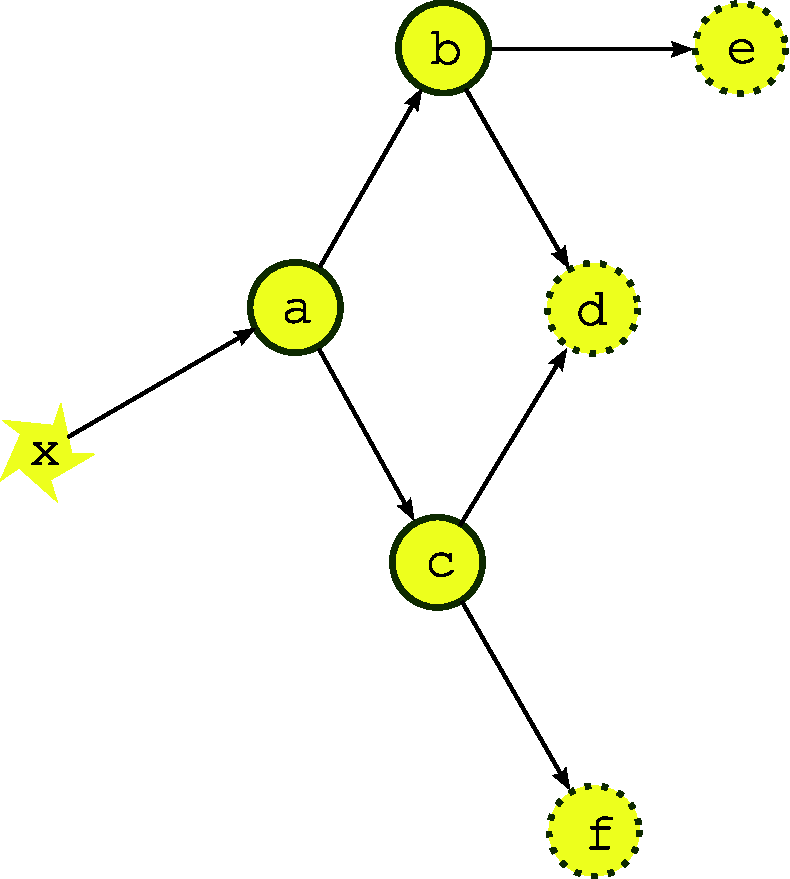
\includegraphics[width=6cm]{inkscape-svg/dep-one-cycle.pdf} 
    \end{center}
    \caption[Single cycle dependency graph for a simple suite]{\small
    The dependency graph for a single forecast cycle of a simple example
    suite. Tasks {\em a, b,} and {\em c} represent forecast models,
    {\em d, e} and {\em f} are post processing or product generation
    tasks, and {\em x} represents external data that the upstream
    forecast model depends on.}
    \label{fig-dep-one} 
\end{figure} 

\begin{figure}
    \begin{center}
        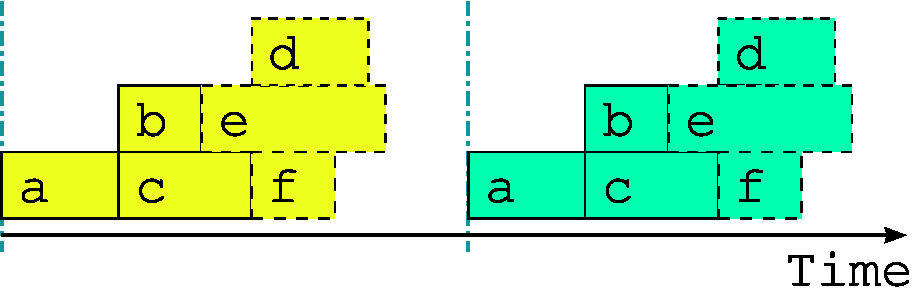
\includegraphics[width=8cm]{inkscape-svg/timeline-one.pdf}
    \end{center}
    \caption[Single cycle job schedules for real time operation]{\small
    The optimal job schedule for two consecutive cycles of our example
    suite during real time operation, assuming that all tasks trigger 
    off upstream tasks finishing completely. The horizontal extent of
    a task bar represents its execution time, and the vertical blue
    lines show when the external driving data becomes available.}
    \label{fig-time-one}
\end{figure}

Figure~\ref{fig-time-one} shows the optimal job schedule for two
consecutive cycles of the example suite in real time operation, given
execution times represented by the horizontal extent of the task bars.
There is a time gap between cycles as the suite waits on new external
driving data.  Each task in the example suite happens to trigger off
upstream tasks {\em finishing}, rather than off any intermediate output
or event; this is merely a simplification that makes for clearer
diagrams.

\begin{figure}
    \begin{center}
        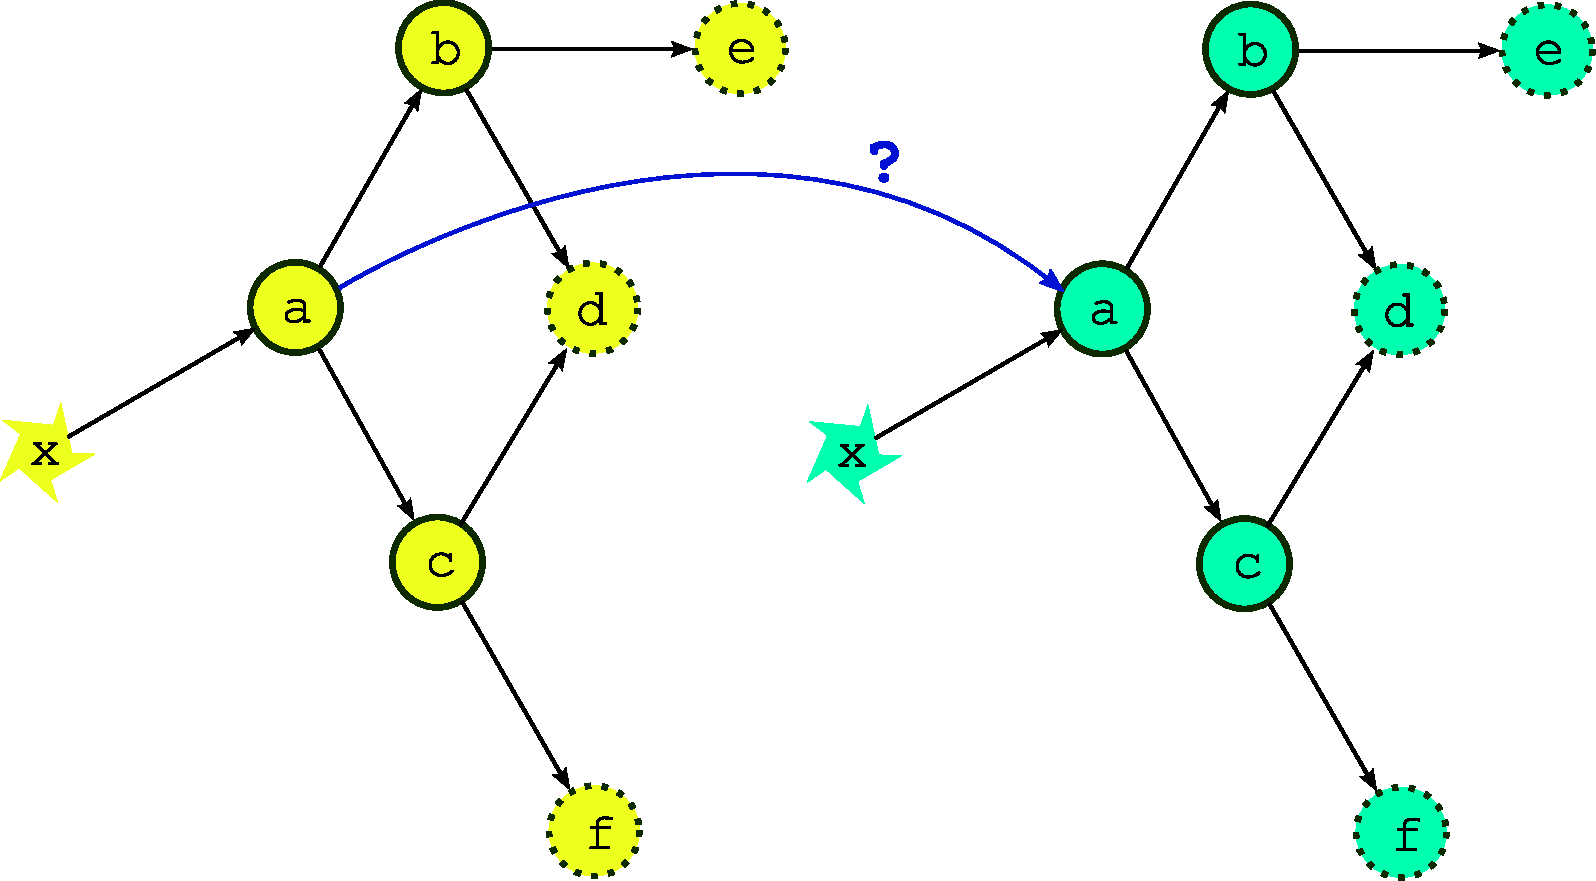
\includegraphics[width=10cm]{inkscape-svg/dep-two-cycles-linked.pdf} 
    \end{center}
    \caption[What if the external data is available early?]{\small If
    the external driving data is available in advance, can we start
    running the next cycle early?} 
    \label{fig-dep-two-linked}
\end{figure}

\begin{figure}
    \begin{center}
        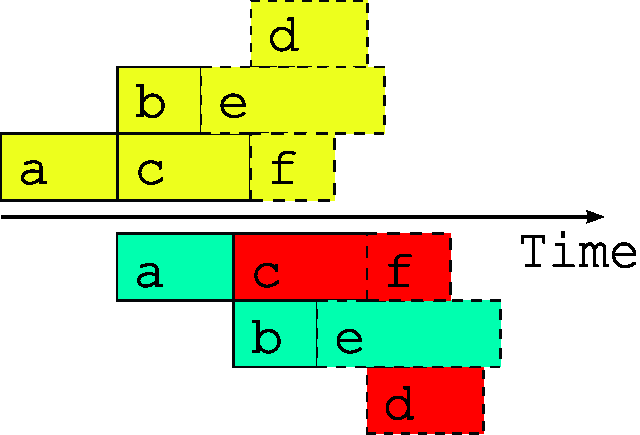
\includegraphics[width=6cm]{inkscape-svg/timeline-one-c.pdf} 
    \end{center}
    \caption[Attempted overlap of consective single-cycle job
    schedules]{\small A naive attempt to overlap two consecutive cycles
    using the single-cycle dependency graph. The red shaded tasks will
    fail because of dependency violations (or will not be able to run
    because of upstream dependency violations).} 
    \label{fig-overlap}
\end{figure} 

\begin{figure}
    \begin{center}
        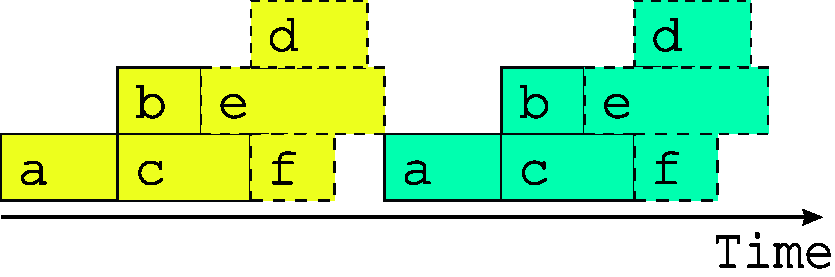
\includegraphics[width=8cm]{inkscape-svg/timeline-one-a.pdf} 
    \end{center}
    \caption[The only safe multicycle job schedule?]{\small The best that
    can be done {\em in general} when intercycle dependencies are
    ignored.} 
    \label{fig-job-no-overlap}
\end{figure} 

Now the question arises, what happens if the external driving data for
upcoming cycles is available in advance, as it would be after a
significant delay in operations, or when running a historical case
study?  While the forecast model {\em a} appears to depend only on the
external data {\em x} at this stage of the discussion, in fact it would 
typically also depend on its own previous instance for the model {\em
background state} used in initializing the new forecast. Thus, as
alluded to in Figure~\ref{fig-dep-two-linked}, task {\em a} could in
principle start
immediately its predecessor has finished.  Figure~\ref{fig-overlap}
shows, however, that starting a whole new cycle at this point is
dangerous - it results in dependency violations in half of the tasks in
the example suite. In fact the situation is even worse than this
- imagine that task {\em b} in the first cycle is delayed for any reason
{\em after} the second cycle has been launched? Clearly we must consider
handling intercycle dependencies explicitly or else agree not to start
the next cycle early, as is illustrated in Figure~\ref{fig-job-no-overlap}.

\subsubsection{Intercycle Dependencies} 
\label{IntercycleDependencies}

In most suites dependencies between tasks in different cycles
exist. Forecast models, as above, typically depend on their own most
recent previous forecast for a background state, and different
types of tasks in different forecast cycles can also be linked (in an 
atmospheric forecast analysis suite, for instance, the weather model 
may also generate background states for use by the observation
processing and data-assimilation systems in the next cycle). In real
time operation these intercycle dependencies
can be ignored because they are automatically satisfied when each cycle
finishes before the next one begins. This is just as well
because they dramatically increase the complexity of the dependency
graph of even the simplest suites, by destroying the clean boundary
between forecast cycles. Figure~\ref{fig-dep-multi} illustrates the
problem for our simple example suite assuming the minimal likely
intercycle dependence: the forecast models ($a$, $b$, and $c$) each
depend on their own previous instances.

For this reason, and because we tend to imagine that forecasting suites
always run in distinct cycles, existing metaschedulers (as far as the author
is aware!) ignore intercycle dependencies and therefore {\em require} a
series of distinct cycles at all times. While this does not affect
normal real time operation it can be a serious impediment when advance
availability of external driving data makes it possible, in principle,
to run some tasks from upcoming cycles before the current cycle is
finished - as suggested at the end of the previous section. This occurs
after delays (late arrival of external data, system maintenance, etc.)
and, to an even greater extent, in historical case studies, and parallel
test suites that are delayed with respect to the main operation. It is
a serious problem, in particular, for suites that have little downtime
between forecast cycles and therefore take many cycles to catch up
after a delay. Without taking account of intercycle dependencies, the
best that can be done, in general, is to reduce the gap between cycles
to zero as shown in Figure~\ref{fig-job-no-overlap}. A limited crude
overlap of the single cycle job schedule may be possible for specific
task sets but the allowable overlap may change if new tasks are added,
and it is still dangerous: it amounts to running different parts of a
dependent system as if they were not dependent and as such it cannot be
guaranteed that some unforeseen delay in one cycle, after the 
next cycle has begun, (e.g.\ due to resource contention or task
failures) won't result in dependency violations.

\begin{figure}
    \begin{center}
        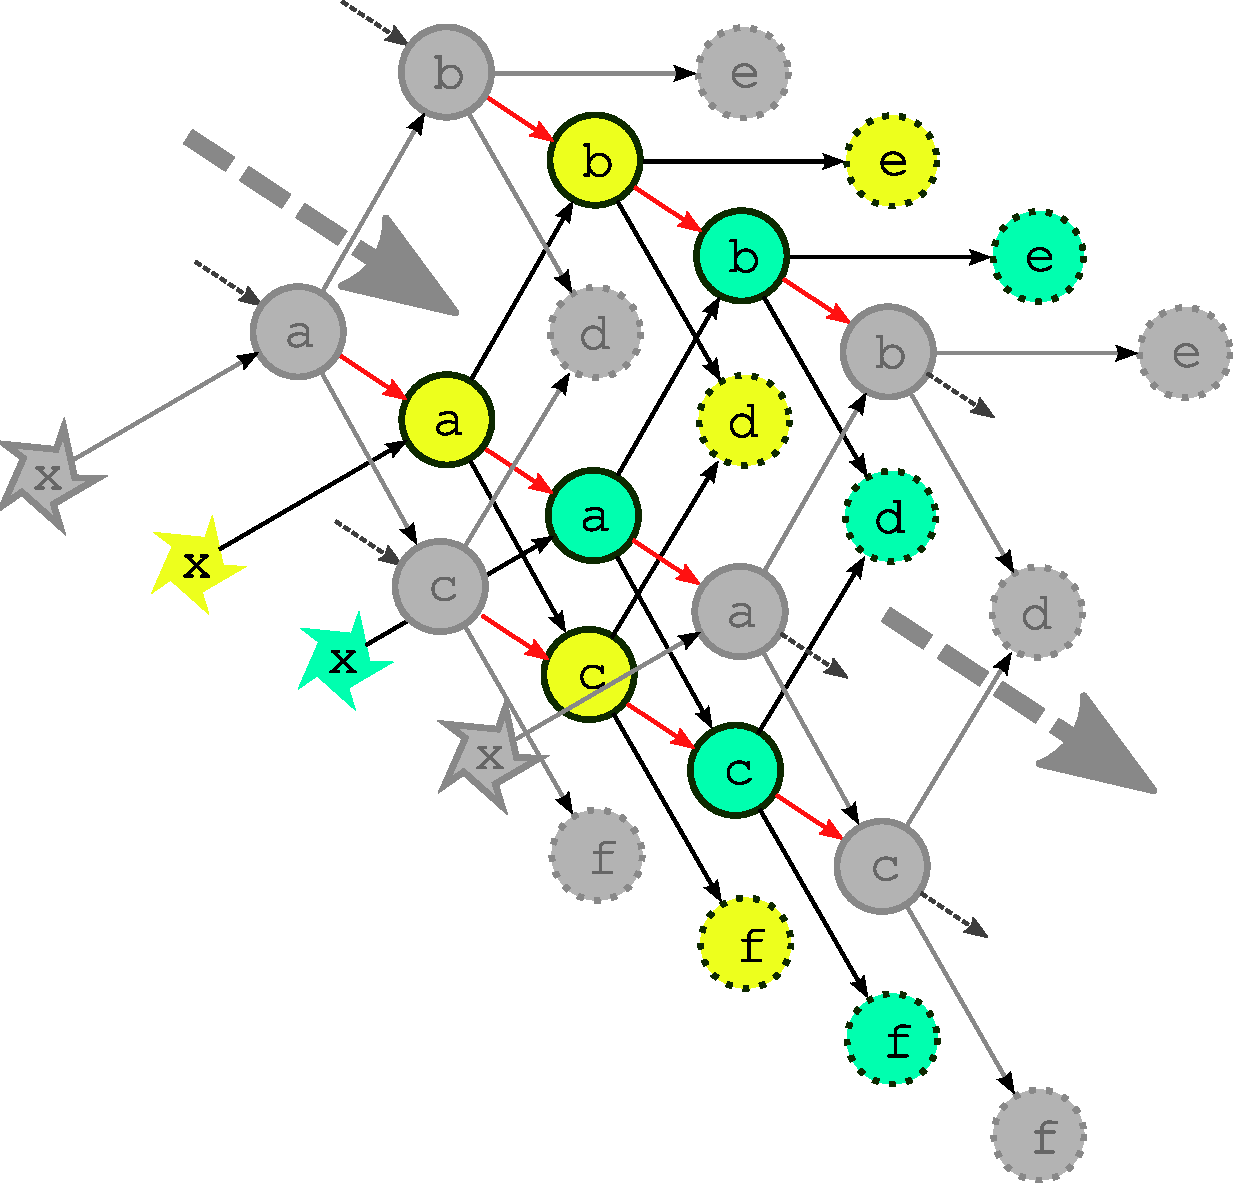
\includegraphics[width=8cm]{inkscape-svg/dep-multi-cycle.pdf} 
    \end{center}
    \caption[Complete multicycle dependency graph]{\small The complete
    dependency graph for the example suite, assuming the least possible
    intercycle dependence: the forecast models ($a$, $b$, and $c$)
    depend on their own previous instances. The dashed arrows show
    connections to previous and subsequent forecast cycles.} 
    \label{fig-dep-multi}
\end{figure}

\begin{figure}
    \begin{center}
        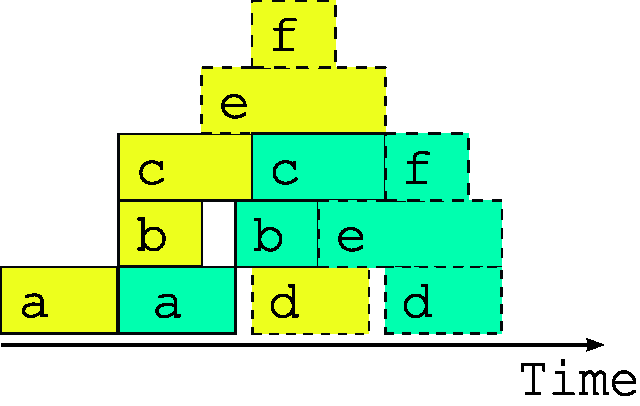
\includegraphics[width=6cm]{inkscape-svg/timeline-two-cycles-optimal.pdf} 
    \end{center}
    \caption[Optimal two-cycle job schedule]{\small Optimal two cycle
    job schedule when the next cycle's driving data is available in
    advance, possible in principle when intercycle dependencies are
    handled explicitly.} 
    \label{fig-optimal-two}
\end{figure} 

Figure~\ref{fig-optimal-two} shows, in contrast to
Figure~\ref{fig-overlap}, the optimal two cycle job schedule obtained by
respecting all intercycle dependencies.  This assumes no delays due to
resource contention or otherwise - i.e.\ every task runs
as soon as it is ready to run. The scheduler running
this suite must be able to adapt dynamically to external conditions 
that impact on multicycle scheduling in the presence of
intercycle dependencies or else, again, risk bringing the system down
with dependency violations.

\begin{figure}
    \begin{center}
        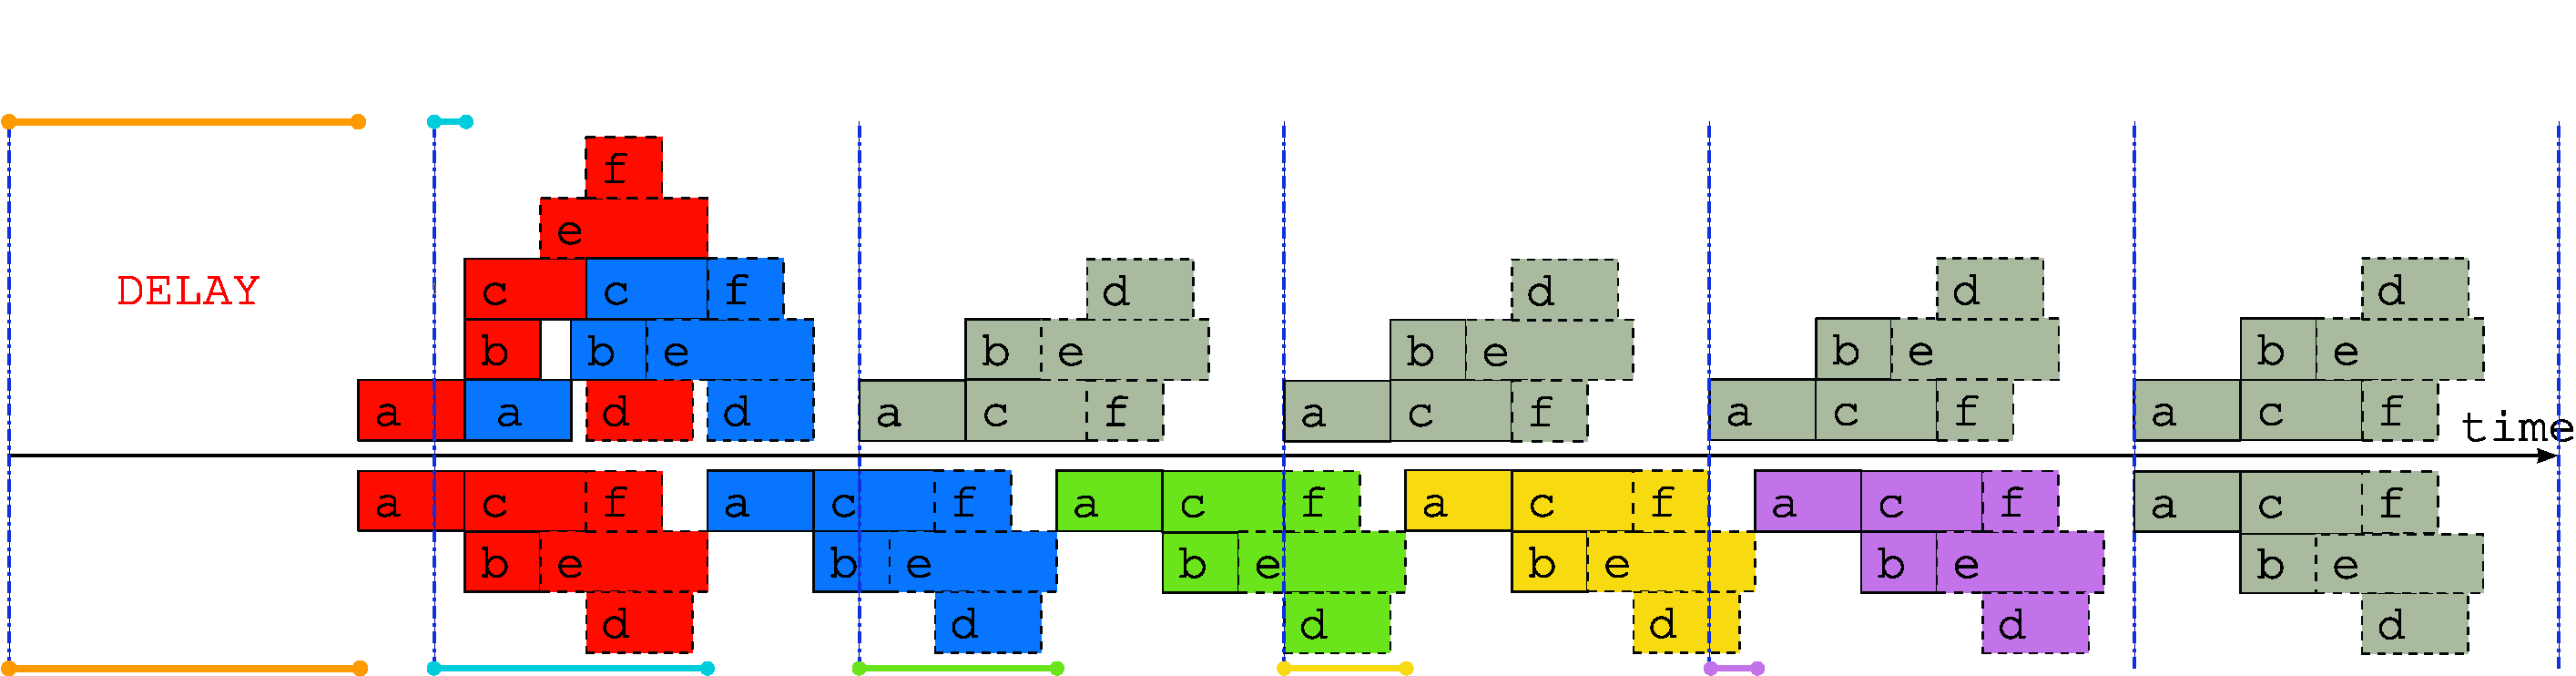
\includegraphics[width=12cm]{inkscape-svg/timeline-three.pdf} 
    \end{center}
    \caption[Post delay comparison of job schedules]{\small Job
    schedules for the example suite after a delay of almost one whole
    forecast cycle, when intercycle dependencies are
    taken into account (above the time axis), and when they are not
    (below the time axis). The colored lines indicate the time that
    each cycle is delayed, and normal ``caught up'' cycles
    are shaded gray.} 
    \label{fig-time-three}
\end{figure} 

\begin{figure}
    \begin{center} 
        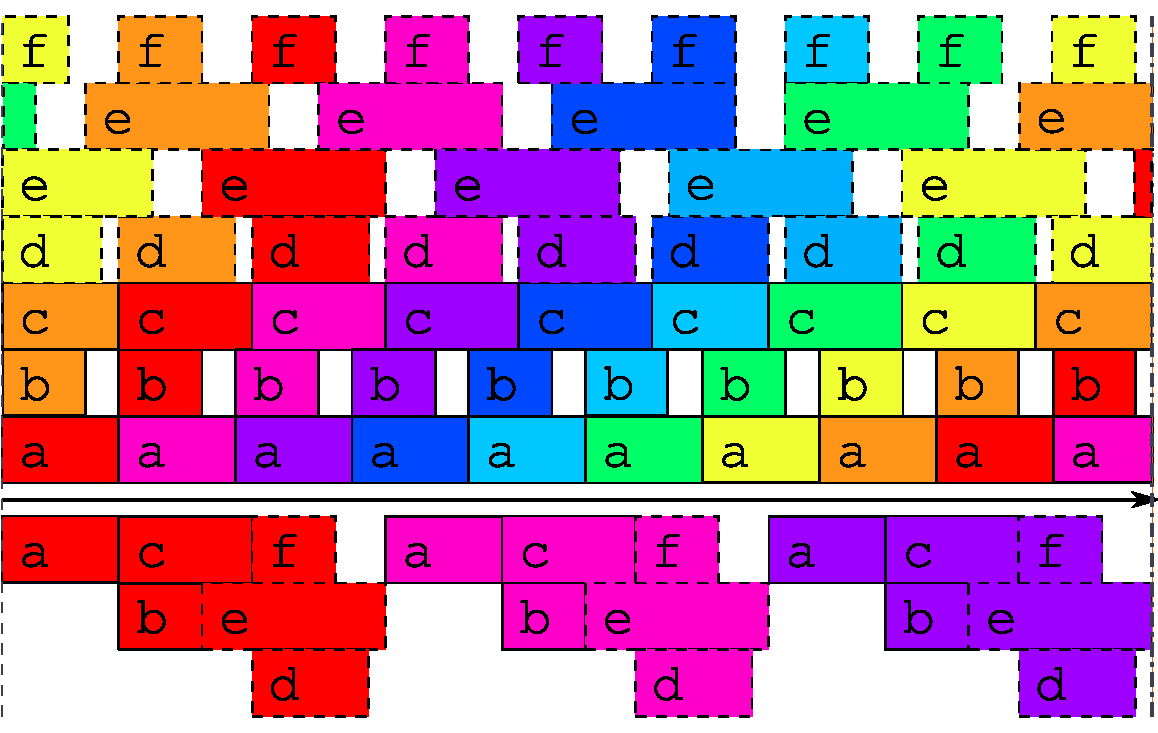
\includegraphics[width=8cm]{inkscape-svg/timeline-two.pdf}
    \end{center} 
    \caption[Optimal job schedule when all external data is
    available]{\small Job schedules for the example suite in case study
    mode, or after a long delay, when the external driving data are
    available many cycles in advance. Above the time axis is the optimal
    schedule obtained when the suite is constrained only by its true
    dependencies, as in Figure \ref{fig-dep-two-linked}, and underneath
    is the best that can be done, in general, when intercycle
    dependencies are ignored.} 
    \label{fig-time-two}
\end{figure} 

To further illustrate the potential benefits of proper intercycle
dependency handling, Figure~\ref{fig-time-three} shows an operational
delay of almost one whole cycle in a suite with little downtime between
cycles. Above the time axis is the optimal schedule that is possible, in
principle, when intercycle dependencies are taken into account, and
below is the only safe schedule possible {\em in general} when they are
ignored.  In the former case, even the cycle immediately after the delay
is hardly affected, and subsequent cycles are all on time, whilst in the
latter case it takes five full cycles to catch up to normal real time
operation.
%Note that simply overlapping the single cycle schedules of
%Figure~\ref{fig-time-one} from the same start point would have resulted
%in dependency violation by task {\em c}.

Similarly, Figure~\ref{fig-time-two} shows example suite job schedules
for an historical case study, or when catching up after a very long
delay; i.e.\ when the external driving data are available many cycles in
advance.  Task {\em a}, which as the most upstream forecast model is
likely to be a resource intensive atmosphere or ocean model, has no
upstream dependence on cotemporal tasks and can therefore run
continuously, regardless of how much downstream processing is yet to be
completed in its own, or any previous, forecast cycle (actually, task
{\em a} does depend on cotemporal task {\em x} which waits on the
external driving data, but that returns immediately when the external
data is available in advance, so the result stands). The other forecast
models can also cycle continuously or with short gap between, and some
post processing tasks, which have no previous-instance dependence, can
run continuously or even overlap (e.g.\ {\em e} in this case). Thus,
even for this very simple example suite, tasks from three or four
different cycles can in principle run simultaneously at any given time. 
In fact, if our tasks are able to trigger off internal outputs of 
upstream tasks, rather than waiting on full completion, successive
instances of the forecast models could overlap as well (because model
restart outputs are generally completed early in the forecast) for an
even more efficient job schedule. 

%Finally, we note again that a good job scheduler should be able to
%dynamically adapt to delays in any part of the suite due to resource
%contention, varying run times, or anything else that will inevitably
%modify the depicted job schedules. 

\subsection{The Cylc Scheduling Algorithm} 
\label{TheCylcSchedulingAlgorithm}

\begin{figure}
    \begin{center} 
        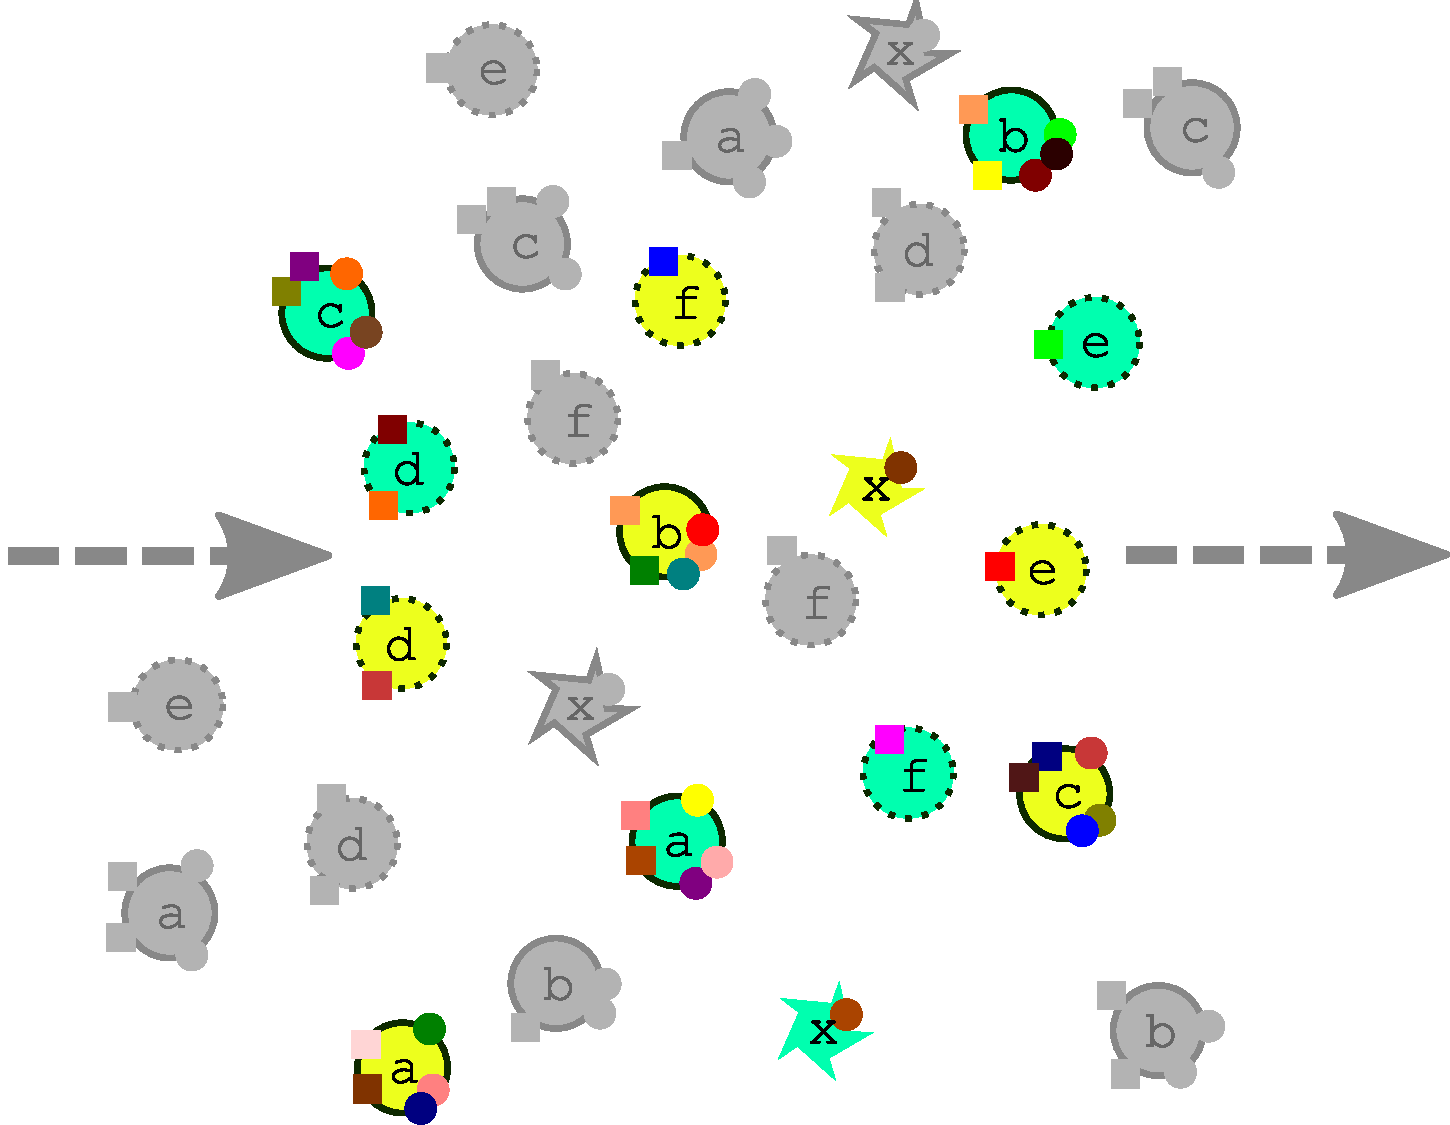
\includegraphics[width=8cm]{inkscape-svg/task-pool.pdf}
    \end{center} 
    \caption[The cylc task pool]{\small How cylc sees the task pool, in
    contrast to the full dependency diagram of Figure~\ref{fig-dep-multi}.} 
    \label{fig-task-pool}
\end{figure} 

This section explains how cylc achieves the optimal multicycle
scheduling described above. 

Cylc manages a pool of proxy objects that represent real tasks in the
forecasting suite. A task proxy object can run the real task when its
prerequisites are satisfied, and can receive reports of completed
outputs from the real task as it runs. There is no global cycling
mechanism to advance the suite in time; instead each individual task
proxy has a private cycle time and spawns its own successor at the right
time (which depends only on the task's own type and state). Task proxies
are self-contained and do not know what other tasks exist in the suite,
they just know their own prerequisites and outputs. Intercycle
dependencies are not treated specially, and the task pool
can be populated with tasks from many different cycle times. Now,
whenever any task proxy changes state (as a result of an output
completion message, for example) cylc gets the entire pool to interact
indiscriminately ({\em regardless of cycle time}) in an attempt to
match unsatisfied prerequisites with completed outputs.\footnote{In fact
this dependency negotiation goes through a middleman or broker object,
which reduces the interaction scaling from $n^2$ to $n$, where $n$ is
the number of task proxies in the suite.} 

Thus without using global cycling mechanisms, and treating all
dependencies equally, cylc in effect gets a set of individual tasks to
self-organise by negotiating their own dependencies: optimal scheduling,
as illustrated in the previous section, emerges naturally at run time.

In addition, cylc makes no distinction between delayed and real time
operation. In delayed operation the tasks that gather the suite's
external driving data will return immediately (because the data is
already available) and the suite will only be constrained by its
internal dependencies. In real time operation, the data gathering tasks
will return only when the external data becomes available (at
some defined offset with respect to the task's cycle time), delaying
downstream tasks until then, by which time the previous forecast cycle
will have completed. A cylc suite thus transitions seamlessly from
optimal multicycle scheduling to a sequence of distinct forecast cycles
as it catches up to real time operation.

%Perhaps the most difficult problem encountered during cylc
%implementation was how to arrange that every task proxy object exists by
%the time it is needed, but not too much earlier, and does not die too
%long after it is no longer needed. This engendered no small amount
%of hair pulling and teeth gnashing, but once achieved the complexities
%therein are entirely hidden from the user.

\pagebreak
\section{Installing Cylc} 
\label{InstallationAndTesting}

\subsection{Requirements} 
\label{Requirements}

\begin{myitemize}
    \item Operating System: Linux or Unix \footnote{The cylc codebase
        assumes Unix-style file paths in places, but it could easily
        made more portable if necessary.} 
    \item Python Version: 2.4 or later, but not Python
        3.x as yet.\footnote{Python 2.4 was released in November 2004. Python 3
        is the future of Python, but it is not backward compatible with
        2.x and consequently still has significantly less library and
        third party support.  As of mid 2011, Python 2.7 is still the
        standard for new Linux distributions.}
    \item Pyro 3 (Python Remote Objects) - latest version test
        3.12.\footnote{As of April 2011, Pyro 4, which is compatible
        with Python 3, is in development but it is still not recommended
        for production use.} Open source license: MIT.
    \item The graphviz graph layout engine (latest version tested:
        2.26.3). Open source license: Eclipse Public License v1.0.
    \item Pygraphviz, a python interface to graphviz (latest version
        tested: 1.0rc6). Open source license: BSD
\end{myitemize}

The software above is required by cylc, but is not part of cylc. Python
and Pyro are absolutely essential. Graphviz and pygraphviz are required
for dependency graph plotting and the graph-based suite control
interface, but you can run cylc without them.

Cylc has also absorbed, in modified form, the following open source
software packages:
\begin{myitemize}
    \item The xdot graph viewer software (open source license: LGPL)
    \item The ConfigObj and Validate python modules (open source license: BSD)
\end{myitemize}


\subsection{Installation} 
\label{Installation}

\subsubsection{Cylc}

Cylc is designed to be installed into a normal user account (called
`admin' below). Simply unpack the cylc release tarball into your chosen
location. Users gain access by sourcing the cylc environment script:

\begin{lstlisting}
# configure your shell environment for access to cylc
admin> export CYLC_DIR=/path/to/cylc/installation/
admin> . $CYLC_DIR/environment.sh
\end{lstlisting}

Note that the variable \lstinline=$CYLC_DIR= is actually required by
the environment script (you can't just skip that step and source the
script directly).

For a system-level install just inspect the environment script for the
few critical executable and source module paths, and install the
contents therein in standard system locations. Users would then not need
to source the cylc environment script before using cylc. 

\subsubsection{Other}

Pyro, graphviz, and Pygraphviz all have their own simple installation
instructions.  If you can't get these installed at system level it is 
quite possible to install them all into a user account, and then adapt
the cylc environment script slightly to ensure that cylc can access 
them.

\subsection{Create the Central Suite Database}

Cylc suites must be registered in a local (user-specific) database 
before they can be used. Suites can also be exported to a central
database visible to all users. Run the following script to 
create the central database and export several example suites to
it:

\begin{lstlisting}
admin> create_cdb.sh
\end{lstlisting}

(You must have installed cylc and configured your environment as above
before doing this).

\subsection{Testing}
\label{Testing}

\subsubsection{Suite Database Test} 

The script \lstinline=$CYLC_DIR/test/test-db.sh= gives
the suite database functionality a work out - it registers the userguide
example suite under a new name and then manipulates it (by copying the
suite in various ways, exporting it to the central database, and so on,
before finally deleting the test registration). This process should
complete in a few seconds.

\subsubsection{Suite Scheduler Test} 

The script \lstinline=$CYLC_DIR/test/test-suite.sh= tests the cylc 
scheduler itself by running an example suite, configuring it 
to fail out a specific task, and then doing some advanced failure
recovery intervention on it (recursive purge). This process
should complete in 2-3 minutes, and can be watched in real time by
firing up a gcylc suite controller instance.

\pagebreak
\section{Quick Start Guide} 
\label{QuickStartGuide}

\lstset{language=bash}

This is an introduction to basic cylc functionality using the example
suite illustrated in the first chapter, which should have been
registered in the central suite database during cylc installation  as
``examples:userguide''. For more detailed information on available
commands and options refer to \lstinline=cylc help= or the {\em Command
Reference} (Appendix~\ref{CommandReference}), gcylc help menus, and
upcoming chapters of this document. 

{\bf For the most part, only the cylc commandline is used in this
chapter, but cylc also has a graphical interface, gcylc, with which you
can do everything from copying, searching, editing, and validating suite
definitions; through to starting, interrogating, and intervening in the
operation of running suites:}

\begin{lstlisting}
prompt> gcylc &                  # generic suite database viewer.
prompt> gcylc [-g] group:name &  # to control a named suite.
\end{lstlisting}

The gcylc modus operandi, in addition to the usual top menu bar, is:
{\em right-click on suites in the database viewer, and on tasks in the
suite control interface, to get a popup menu of available options}.

\subsection{Configure Your Environment For Cylc}

To gain access to cylc you just need to source the cylc environment
script. Put the following in your login script, or do the same at the
terminal prompt before using cylc.\footnote{To switch between different
cylc installations on the same host, just source the appropriate 
environment script.}
\begin{lstlisting}
prompt> export CYLC_DIR=/path/to/cylc/installation
prompt> . $CYLC_DIR/environment.sh
\end{lstlisting}

You should also specify the graphical and terminal editors you want to
use to edit suites, by setting the following environment variables in
your \lstinline=.profile=:
\begin{lstlisting}
export GEDITOR='gvim -f'  # GUI editor launched by gcylc
export EDITOR=vim         # terminal editor launched by 'cylc edit'
\end{lstlisting}
(see \lstinline=cylc edit help= for other tested editors).

\subsection{Start Your Lockserver Daemon}

Each cylc user should run a lockserver to prevent accidental 
invocation of multiple instances of the same suite or task at the same 
time.  The suite and task locks brokered by the lockserver are analogous
to traditional lock files, but they work across a network, even for
distributed suites containing tasks that start executing on one host and
finish on another.

The lockserver daemon can be started at any time and left running.
\begin{lstlisting}
prompt> cylc lockserver start
\end{lstlisting}

Check that it is running,
\begin{lstlisting}
prompt> cylc lockserver status
\end{lstlisting}

For detailed usage information,
\begin{lstlisting}
prompt> cylc lockserver --help 
\end{lstlisting}

There is a command line client interface, 
\lstinline=cylc lockclient=,
for interrogating the lockserver and managing 
locks manually (c.f.\ having to delete a lock file manually when the
associated process died without cleaning up after itself).

You can also choose not to use the lockserver for a particular suite, by
setting the following switch in its suite.rc (suite
definition) file,
\begin{lstlisting}
# SUITE.RC:
use lockserver = False  # not recommended!
\end{lstlisting}

\subsection{Copy The Example Suite} 

Now we'll import the example suite from the central database to,
\begin{lstlisting}
$HOME/cylc/examples/userguide
\end{lstlisting}
and register it as,
\begin{lstlisting}
examples:userguide
\end{lstlisting}

\subsubsection{using gcylc}

Start gcylc, switch to the central database view, right-click on
\lstinline=admin > examples > userguide= 
(where `admin' is the username of the cylc installation account),
choose `Import', and specify the registration GROUP and NAME, and 
destination path, as above. Check that the import was successful
by inspecting the command output window, and switching the view back to
your local database, which should now contain your copy of the suite.

\subsubsection{using the commandline}

Check that the example suite is registered in the central database,

\begin{lstlisting}
prompt> cylc db print --central | grep userguide # or:
prompt> cylc db print --central --group=examples --name=userguide
admin:examples:userguide  "userguide example suite" \
    /home/admin/cylc/examples/userguide
\end{lstlisting}

Now import the suite,
\begin{lstlisting}
prompt> cylc db import admin:examples:userguide $HOME/cylc/examples/userguide
\end{lstlisting}

Check that the import was successful,
\begin{lstlisting}
prompt> cylc db print | grep userguide # or:
prompt> cylc db print --group=examples --name=userguide
examples:userguide "userguide example suite" /home/oliverh/cylc/examples/userguide
\end{lstlisting}

You can now edit, search, validate, plot, run, etc., your copy of the
example suite, using the commandline or gcylc (right-click on the suite
as described above). On the commandline type \lstinline=cylc help= and
drill down to the command you want.

\subsection{Searching, Editing, and Plotting the Suite}

In gcylc, right-click on the suite and choose `Edit'; 
Right-click again and choose 'Graph' to plot the suite dependency graph
defined in the suite.rc file. You'll need to enter an initial and final
cycle time (YYYYMMDDHH) for the plot range - enter the same cycle time
for both to plot a single cycle.  If you edit the dependency graph, the
viewer should update when you save the suite.rc file.

To edit a suite from the commandline,
\begin{lstlisting}
prompt> cylc edit examples:userguide
\end{lstlisting}
This moves to the suite definition directory (so that you can easily
open other suite files in the same edit session) and opens the
suite.rc file in your chosen editor. You can of course
do this entirely manually, but using the edit command has some advantages. 
For example, you don't have to remember the suite definition directory
location, and for suite.rc files that contain include files
(even nested ones) you can optionally edit the file inlined - it will be
split back into include-files {\em when you save and exit the editor}. 

To graph the suite,
\begin{lstlisting}
prompt> cylc graph examples:userguide 2011042506 2011042606 &
\end{lstlisting}

And here's how to use the suite search tool, which reports matches in
the suite.rc by line number, suite section, and file (even
if nested include-files are used) and by file and line number for
matches in the suite bin directory,

\begin{lstlisting}
prompt> cylc grep OUTPUT_DIR examples:userguide

FILE: /home/oliverh/cylc/examples/userguide/suite.rc
   SECTION: [tasks]->[[X]]->[[[environment]]]
      [53]:             OUTPUT_DIR = $WORKSPACE
   SECTION: [tasks]->[[A]]->[[[environment]]]
      [59]:             OUTPUT_DIR = $WORKSPACE

<...snip...>

FILE: /home/oliverh/cylc/examples/userguide/bin/E.sh
   [7]: cylc checkvars -c OUTPUT_DIR
   [21]: touch $OUTPUT_DIR/sea-state.products

FILE: /home/oliverh/cylc/examples/userguide/bin/D.sh
   [7]: cylc checkvars -c OUTPUT_DIR
   [24]: touch $OUTPUT_DIR/combined.products

<...snip...>
\end{lstlisting}

See the gcylc right-click menu, or \lstinline=cylc prep help= for other
commands in the ``suite preparation''.

Note that the suite title held by the database is only parsed from the
suite.rc file at registration time; if you change the title
use \lstinline=cylc db refresh= or gcylc 
\lstinline=View > Refresh= to update the database.

After editing a suite, always validate it to check for errors prior to
running it (gcylc right-click or \lstinline=cylc validate SUITE:GROUP=)

\subsection{Running The Suite}

\begin{lstlisting}
cylc run userguide 2011042506
\end{lstlisting}

You should now start up a suite control interface to follow progress.
\begin{lstlisting}
gcylc examples:userguide &
\end{lstlisting}

Or, if you already have the gcylc database front end running, right click on the 
suite and choose one of the `Control' options.  Note 
that the control GUI can also be used to start and stop the suite.

In real mode operation (as opposed to {\em dummy mode},
Section~\ref{DummyMode}) {\em do not choose an initial cycle time in the
future} or nothing will happen until that time arrives!

The lockserver will let you run multiple instances of the userguide
example suite at once, under different registrations, because the
suite.rc file allows that (in turn, because the suite
group:name is used in all I/O file paths).

%\begin{figure}
%    \begin{center}
%        %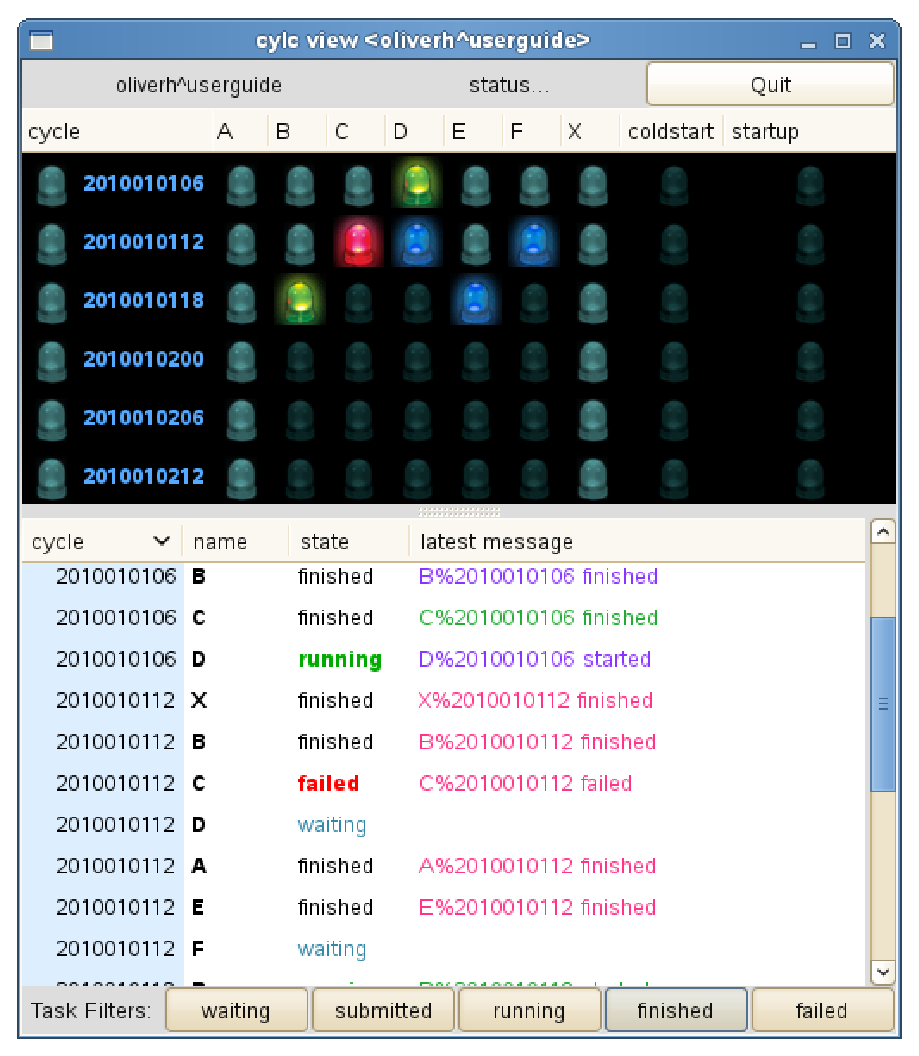
\includegraphics[width=12cm]{monitor} 
%        %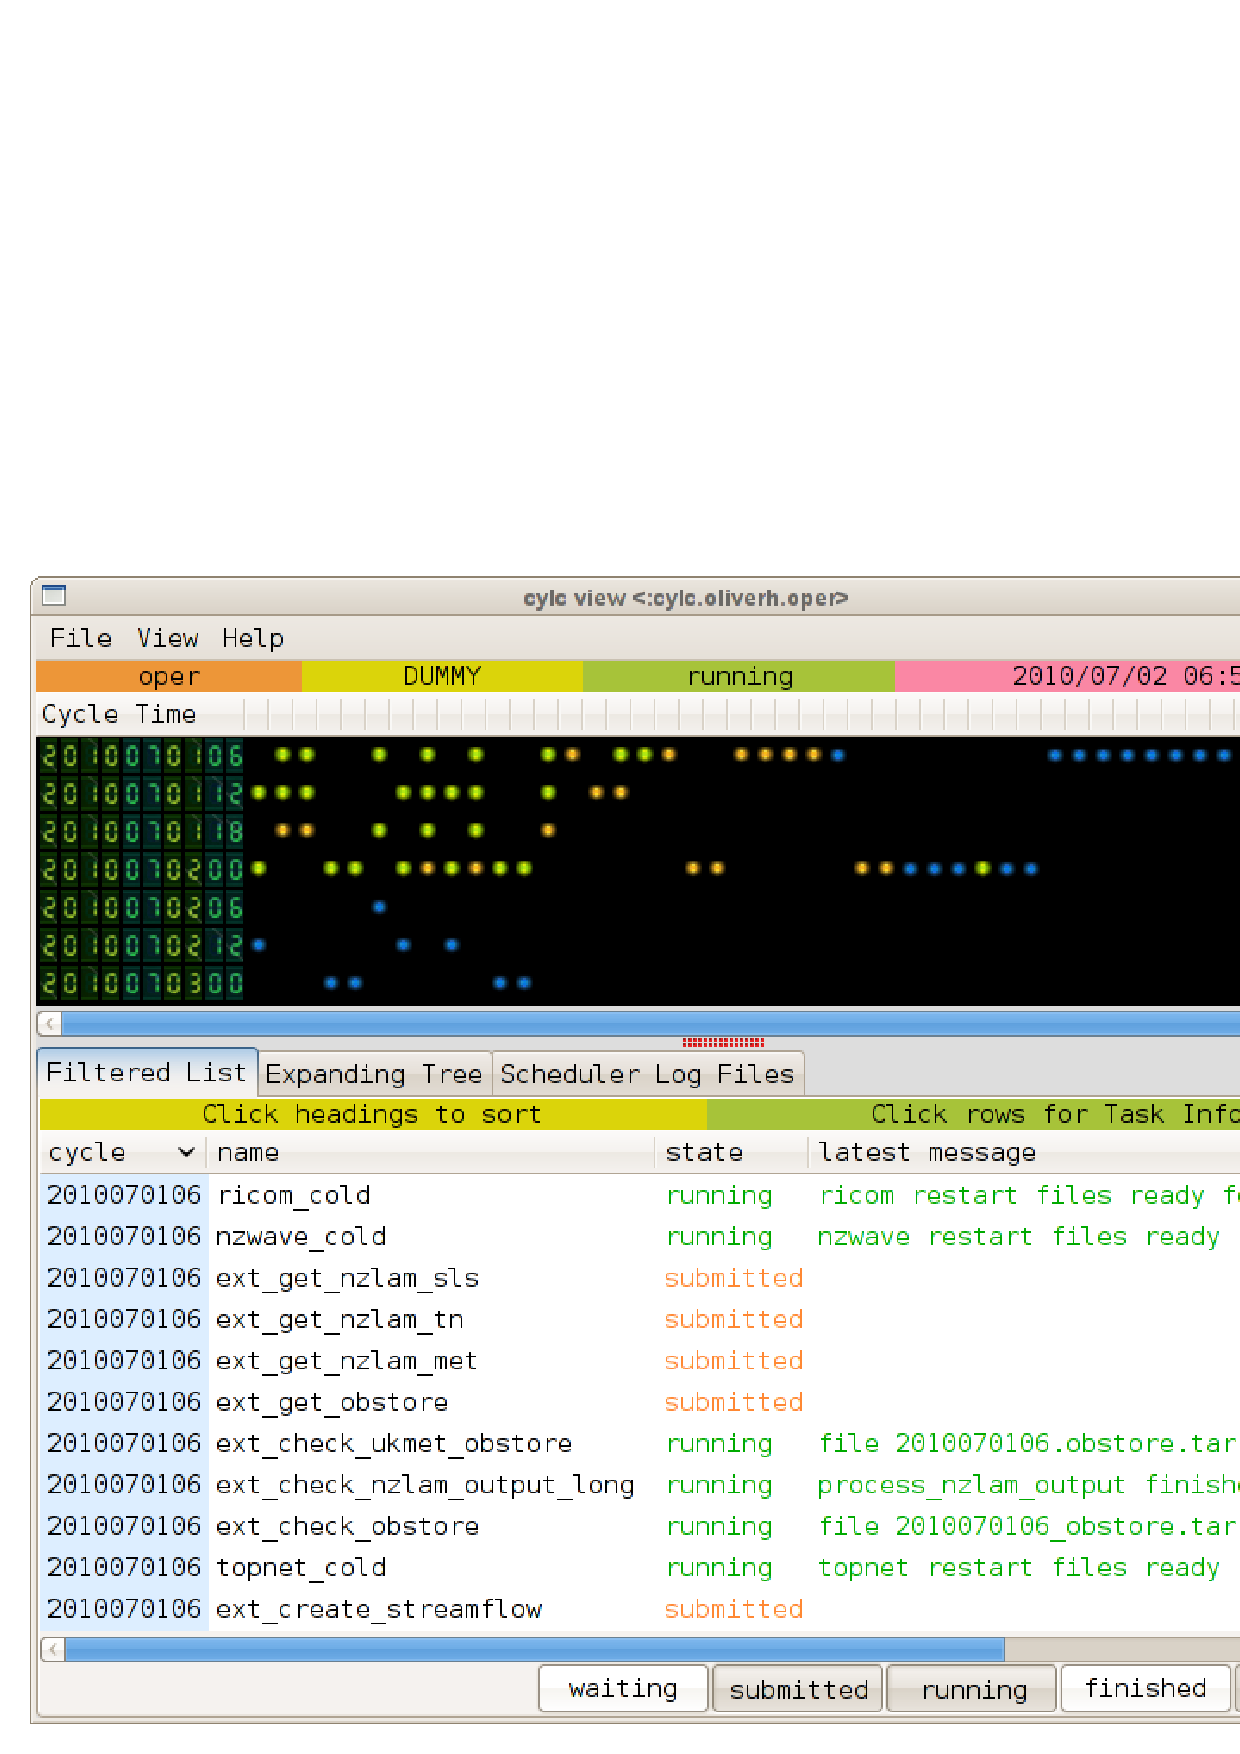
\includegraphics[width=12cm]{cylc-view-ecoconnect.pdf} 
%    \end{center}
%    \caption{\small {\em cylc view} screenshot}
%    \label{fig-monitor} 
%\end{figure} 

\subsection{Shutdown And Restart}

\lstset{language=bash}

\begin{lstlisting}
cylc stop userguide
\end{lstlisting}

This will cause the suite to stop once any currently running tasks have finished. To stop
the suite immediately use the \lstinline=--now= option, but be aware that this will 
orphan any tasks that are still running.  

You can now restart the  suite from its most recent previous state, if you like:
\begin{lstlisting}
cylc restart userguide
\end{lstlisting}
or from the state recorded in a particular named state dump file 
(cylc automatically dumps extra time-stamped state files prior to any
suite intervention so that you can easily revert to the
pre-intervention state in case of disaster). See {\em Restarts}
(Section~\ref{Restarts}) for more information.

\pagebreak

\section{Suite Design} 
\label{SuiteDesign}

\subsection{History}
\subsubsection{Cylc pre-3.0}

Early versions of cylc were focused on developing and testing the new 
scheduling algorithm, and the suite design interface at the time was
essentially the quickest route to that end. A suite was a collection
of ``task definition files'' that encoded the prerequisites and outputs
of each task in a direct reflection of cylc's internal task proxies. 
This way of defining suites exposed cylc's self-organising nature to the
user, and it did have some nice properties. For instance a group of
tasks could be transferred directly from one suite to another by simply
copying the taskdef files over (and checking that prerequisite and
output messages where consistent with the new suite). However, ensuring
consistency of prerequisites and outputs across a large suite could be
tedious; a few edge cases associated with suite startup and forecast
model restart dependencies were, arguably, difficult to understand; and
the global structure of a suite was not readily apparent until run time
(although to counter this cylc could generate run-time resolved
dependency graphs very quickly in dummy mode).

\subsubsection{Cylc post-3.0}

At version 3.0 we implemented an entirely new suite design interface
that, in essence, defines the suite dependency graph and the commandline
and execution environment for each task, in a single, structured,
validated, config file (suite.rc).  This {\em really} makes suite
structure apparent at a glance, and task prerequisites and outputs (and
other important parameters besides) no longer need to be specified by
the user because they are implied by the graph.


\subsection{Suite Definition Directories}

A cylc {\em suite definition directory} contains, at the least, a
suite.rc file (the suite definition) and a \lstinline=bin= sub-directory
(scripts and programs that implement, or are used by, suite tasks).

\begin{lstlisting}
/path/to/my/suite   # suite definition directory

    suite.rc           # ! SUITE DEFINITION !

    bin/               # bin directory (scripts, programs)
        foo.sh
        bar.sh
        ...

    # (OPTIONAL) any other suite-related files, for example:
    inc/               # suite.rc include-files
        nwp-tasks.rc
        globals.rc
        ...
    doc/               # documentation
    control/           # control files
    ancil/             # ancillary files
    ...
\end{lstlisting}

Strictly speaking the suite bin directory is optional because every task
could, in principle, call external commands, scripts, or programs.
However, tasks automatically get access to their suite bin directory,
and there are definite advantages to keeping everything in one place.

Aside from the suite.rc file and bin directory, you can store anything
you like in the suite definition directory - documentation,
configuration data, control files, etc. These will ignored by cylc but
can be accessed by tasks via the \lstinline=$CYLC_SUITE_DIR= variable
that is exported into the execution environment of every task. {\em
Holding everything suite-related in the one place makes suite revision
control easy and powerful.}

\subsection{suite.rc Files}
\label{SuiteRCFile}

Cylc suite definition is handled by a somewhat modified version of
the powerful open source {\em ConfigObj} and {\em Validate}
modules.\footnote{http://www.voidspace.org.uk/python/configobj.html,
BSD licence. Cylc modifies ConfigObj to allow continuation lines and
include-files, and variable overrides in task environment and directives
sections.} Cylc suite.rc files are automatically validated
against a specification, and they translate directly into nested
dictionary data structures inside the program - making it very
easy to add new configuration items to cylc.

\begin{myitemize}
    \item {\bf All Entries} are of the form \lstinline@item = value@.
    \item {\bf [Section] and [[Subsection]] Headings} use nested square brackets.
    \item {\bf \#Comments} follow a hash character, to the end of the line.
    \item {\bf ``Strings''} are quoted.\footnote{quotes can actually be
        omitted in single line strings, so long they don't contain
        commas, which turn unquoted strings into lists.}
    \item {\bf ``````Multiline \newline Strings''''''} are triple-quoted.
    \item {\bf L,i,s,t,s} are comma separated (and space may follow the comma)
    \item {\bf White Space} is ignored but you can indent for clarity.
    \item {\bf Sections are closed by the next section heading},
        so within a section all top level items must be defined before
        any subsections (and similarly for lower levels of nesting).
\end{myitemize}

And the following are cylc-specific additions to the ConfigObj format:

\begin{myitemize}
    \item {\bf Continuation \textbackslash \newline lines} follow a trailing backslash.
    \item {\bf Dependency Graph Strings} may contain blank lines
        and inline comments (see Section~\ref{SuitercDependencyGraph}).
    \item {\bf Include-files} \lstinline=%include path/to/incfile= -
        paths specified, portably, relative to the suite definition
        directory; they can span section boundaries, and may be
        multiply-included and nested. 
\end{myitemize}

 The following pseudo-listing illustrates the file format:

\begin{lstlisting}
# comment
item = value # trailing comment
a string item = the quick brown fox
another string item = "the quick brown fox"
yet another string item = """the quick brown fox
jumped over the lazy dog"""
a list item = foo, bar, baz
a list item with continuation = a, b, c, \
                                d, e, f
[section]
    item = value
%include inc/vars/foo.inc  # include file

    [[subsection]]
        item = value

        [[[subsubsection]]]
            item = value

[another section]
    [[another subsection]]
        # ...
    # ...
# ...
\end{lstlisting}


\subsubsection{A Simple Example}

This is the suite.rc file defining cylc's {\em ``simple''}
example suite; a few entries have been omitted in order to show the
file's structure clearly:

\begin{lstlisting}
# GLOBAL SETTINGS
title = a simple example suite
job submission method = loadleveler
 
[special tasks]
    # TASKS WITH UNUSUAL BEHAVIOR
    startup         = Prep
    coldstart       = ColdA
    sequential      = ModelA
    clock-triggered = GetData(1)

[dependencies]
    # THE SUITE DEPENDENCY GRAPH
    [[ 0,6,12,18 ]]  # four times daily
        graph  =  """
            Prep => GetData & ColdModel
            GetData => Model => PostA
        # Model depends on its previous f/c, or a cold start f/c:
            ColdModel | Model(T-6) => Model
                  """
    [[ 6,18 ]]  # extra postprocessing at 6 or 18 UTC
        graph = "Model => PostB" 

[environment]
    # ENVIRONMENT VARIABLES AVAILABLE TO ALL TASKS
    WORKSPACE = /$TMPDIR/$CYLC_SUITE_GROUP/$CYLC_SUITE_NAME

[tasks]
    # COMMAND AND EXECUTION ENVIRONMENT FOR EACH TASK
    [[GetData]]
        description = "retrieve data for the current cycle time"
        command = cylc wrap GetData.sh
        [[[environment]]]
            # ENVIRONMENT VARIABLES AVAILABLE TO THIS TASK
            GETDATA_OUTPUT_DIR = $WORKSPACE
    [[Model]]
        # ...
    [[PostA]]
        # ...
    # ...
# ...
\end{lstlisting}

The dependency graph defined here can be plotted by gcylc or the
\lstinline=cylc graph= command, as is shown in Figure~\ref{fig-simple-graph}.

\begin{figure}
\begin{minipage}[t]{0.5\textwidth}
    \begin{center}
        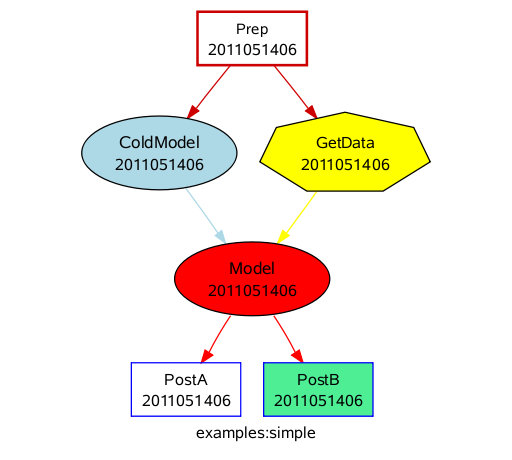
\includegraphics[width=0.4\textwidth]{../images/screenshots/simple-6-cold.png}
    \end{center}
\end{minipage}
\hfill
\begin{minipage}[t]{0.5\textwidth}
    \begin{center}
        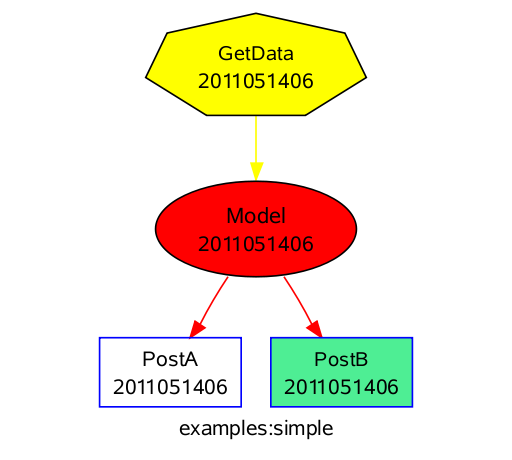
\includegraphics[width=0.4\textwidth]{../images/screenshots/simple-6-warm.png}
    \end{center}
\end{minipage}
\caption[Dependency graphs for the simple example suite]{\small Two dependency graphs
plotted by `cylc graph' from the {\em simple} example suite.rc file; cold
start on the left, warm start on the right.}
\end{figure} 

\begin{figure}
    \begin{center}
        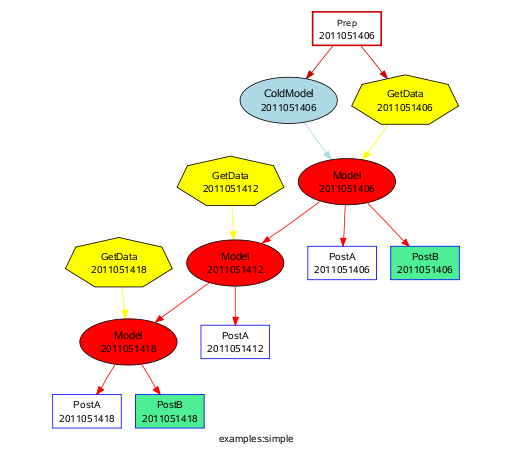
\includegraphics[width=0.8\textwidth]{../images/screenshots/simple-18-cold.png}
    \end{center}
\caption[Three cycle cold start dependency graph for the simple example
suite]{\small Three cycle cold start dependency graph plotted by `cylc
graph' from the {\em simple} example suite.rc file, showing variation between cycles.}
\end{figure} 

\subsubsection{Syntax Highlighting}

The file \lstinline=$CYLC_DIR/conf/cylc.vim= configures 
suite.rc syntax highlighting and section folding for the
{\em vim} editor, as shown in Figure~\ref{fig-cylc-vim}.
To use this, copy the syntax file to your
\lstinline=$HOME/.vim/syntax/= directory and make some minor
modifications, as described in the file, to your
\lstinline=$HOME/.vimrc=.

\begin{figure}
    \begin{center}
        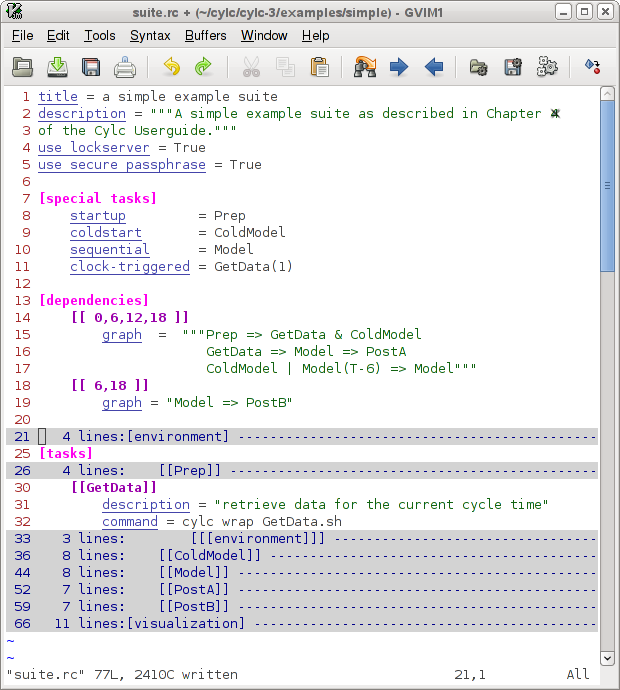
\includegraphics[width=14cm]{../images/screenshots/simple-suiterc.png}]
    \end{center}
    \caption[Cylc suite.rc syntax highlighting in vim]{
    Cylc suite.rc syntax highlighting and folding in the vim editior.}
    \label{fig-cylc-vim} 
\end{figure} 

\subsection{Suite Validation}

Suite validation is designed to catch most suite definition errors
before run time.  First the suite.rc file is validated
against the spec file \lstinline=$CYLC_DIR/conf/suiterc.spec=, which 
is the ultimate arbiter of what's legal in a cylc suite definition
(see Section~\ref{SuiteRCReference}). This detects any formatting
errors, misspelled or illegal items, and illegal values. Then some
cross-entry consistency checking is done. And finally,
an attempt is made to create all of the suite's task proxy objects
according to the information parsed from the suite.rc file.

Here's an example of a successful validation,
\begin{lstlisting}
prompt> cylc validate examples:simple
Parsing Suite Config File
Instantiating Task Proxies:
  -  ColdModel ... OK
  -  GetData ... OK
  -  Model ... OK
  -  PostA ... OK
  -  PostB ... OK
  -  Prep ... OK
Suite examples:simple validates OK.
DONE
\end{lstlisting}

\subsubsection{Suite Definition Errors}

The validator reports line numbers when errors are detected 
(if you use suite.rc include-files, 
the \lstinline=cylc inline SUITE= command, or the gcylc suite 'Edit'
function, makes an inlined copy with correct line numbers):

\begin{lstlisting}
prompt> cylc validate examples:simple
Parsing Suite Config File
ERROR: [[special tasks]
NestingError('Cannot compute the section depth at line 19.',)
_validate examples:simple  failed:  1
\end{lstlisting}

\subsubsection{Suite Definition Warnings}

Several kinds of warning are emitted by the validator, principally 
if any tasks in the dependency graph are not defined in the [tasks]
section, or if any tasks defined in the [tasks] section are not used in
the dependency graph:
\begin{lstlisting}
Parsing Suite Config File
WARNING: task "PostA" is defined only by graph: it will run as a dummy task.
WARNING: task "Prep" is defined in [tasks] but not used in the graph.
Instantiating Task Proxies:
  -  ColdModel ... OK
  -  GetData ... OK
  -  Model ... OK
  -  PostA ... OK
  -  PostB ... OK
  -  Prep ...WARNING: no hours in graph or [tasks][[Prep]]; task can be 
                      'submit'ed but not inserted into the suite.
 OK
Suite examples:simple validates OK.
DONE
\end{lstlisting}

These are not necessarily errors - a task defined by graph alone will
run as a dummy task, and you can temporarily disable a defined task by
commenting it out of the dependency graph. 


\subsection{The Suite Dependency Graph}

\subsubsection{Task Families}

FamilyX = Foo, Bar, Baz

A task family is a group of tasks that behave as a single unit - the
suite triggers the whole group at once, and downstream tasks can trigger
off the group as a whole.

Implementation: the "family" itself is an abstract task type that just
enters the 'running' state when its prerequisites are satisfied; members
automatically trigger off their family starting up; the family's final
state (finished or failed) is not determined until all of its members
have either finished or failed. If *all* members finish successfully the
family enters the 'finished' state, otherwise it enters the 'failed'
state.

Task families can be declared 'sequential', in which case their members 
will run sequentially even if not sequential themselves.

Families can have internal dependencies amongst members, and family 
members can be part of other non-family relationships (e.g. a non-member
task can trigger off a single member rather than the whole group); 
however, the utility of this is not entirely clear. 

{\bf How to recover from a family member (and therefore family) failure:} 
\begin{myitemize}
    \item 1/ fix the problem that caused the failure
    \item 2/ then reset the failed member task to 'waiting' (or retrigger it)
    \item 3/ then reset the family state to 'waiting' (or retrigger it)
\end{myitemize}
When the family triggers again, the reset member task will follow suit. If the
member then completes successfully this time, so will the family, and downstream
processing can proceed as normal.

To trigger downstream processing off a family even if one or more of its 
members failed (e.g.\ a family of obs processing tasks wherein you still
want to use the obs that were successfully processed, even if some were not),
using a conditional trigger:

\begin{lstlisting}
    graph = familyX | familyX:fail => PostProc
\end{lstlisting}


\pagebreak

\section{Cylc Tasks}

A {\em task} is a single schedulable unit in a cylc suite, uniquely
identified by name and cycle time.

\subsection{Task Names}

Tasks are an in-suite abstraction so to rename a task, just change
its name in the suite.rc file (different suites can run the same
processing under different task names).\footnote{Cylc task messaging
commands, which report task progress back to the suite, do need to know
the task name, and the target suite, but they automatically extract this
information from the task execution environment, which is configured by
the suite, so no explicit use of tasks names is required outside of the
suite.rc file.}

\subsection{Task Commandline and Environment}

Every task has an associated commandline that initiates the processing
that it represents. The commandline and the environment in which it
executes is specified for each task in the suite.rc file.

\subsection{Task Job Scripts (How Tasks Are Invoked By Cylc)}

When a task is ready to run, cylc writes, and then executes via the job
submission method specified for the task (see
Section~\ref{JobSubmission}), a {\em job script} that
configures the environment appropriately and then calls the commandline
specified for the task, which in turn executes the {\em task script} 
as described just above.

%In more detail, the temporary ``job script'' contains:
%\begin{myitemize}
%    \item scripting to configure the execution environment for the task
%        This includes user-defined environment variables:
%        \begin{myitemize}
%            \item global environment variables
%            \item task-specific environment variables
%            \item pre- and post-command scripting
%            \item any batch queue scheduler directives
%        \end{myitemize}
%        and cylc-defined environment variables:
%        \begin{myitemize}
%            \item to identify the task and cycle time, etc.
%            \item to portably locate the suite definition directory
%            \item for access to cylc itself
%        \end{myitemize}
%    \item scripting to call the commandline defined for the task.
%\end{myitemize}
        
Cylc writes the exact command used to submit each task to the suite
stdout stream, so you can see the job script location, and
any output redirection used, etc. The following is an excerpt from
example suite stdout, running with the \lstinline=background= job
submission method:

\begin{lstlisting}
# CYLC STDOUT
ColdB%2011101300  READY TO RUN
SUBMITTING TASK: /tmp/cylc-ColdB%2011101300-5gRx61 </dev/null 
    1> /home/oliverh/CylcLogs/examples/userguide/ColdB%2011101300-N3pBYv.out 
    2> /home/oliverh/CylcLogs/examples/userguide/ColdB%2011101300-N3pBYv.err &
\end{lstlisting}

You can also use \lstinline=cylc submit --dry-run= to generate a task
job script for inspection. Here's a simple example:

\begin{lstlisting}
prompt> cylc submit --dry-run examples:userguide A%2010080806 
DRY RUN: create the job script and show how it would be executed.
  * TASK JOB SCRIPT: /tmp/cylc-A%2010080806-VXQusn
  * JOB SUBMISSION METHOD: /tmp/cylc-A%2010080806-VXQusn </dev/null \
    1> /home/oliverh/CylcLogs/examples/userguide/A%2010080806-CWYM68.out
    2> /home/oliverh/CylcLogs/examples/userguide/A%2010080806-CWYM68.err &

prompt> cat /tmp/cylc-A%2010080806-VXQusn
#!/bin/bash

# ++++ THIS IS A CYLC TASK JOB SCRIPT ++++
# Task: A%2010080806
# To be submitted by method: 'background'

# CYLC SUITE ENVIRONMENT:
export CYLC_MODE="submit"
export CYLC_SUITE_HOST="oliverh-33586DL.greta.niwa.co.nz"
export CYLC_SUITE_PORT="NONE"
export CYLC_DIR="/home/oliverh/cylc"
export CYLC_SUITE_DIR="/home/oliverh/cylc/examples/userguide"
export CYLC_SUITE="examples:userguide"
export CYLC_SUITE_GROUP="examples"
export CYLC_SUITE_NAME="userguide"
export CYLC_SUITE_OWNER="oliverh"
export CYLC_USE_LOCKSERVER="True"
export CYLC_DUMMY_SLEEP="10"

# CYLC ENVIRONMENT:
. $CYLC_DIR/environment.sh

# TASK IDENTITY:
export TASK_ID=A%2010080806
export TASK_NAME=A
export CYCLE_TIME=2010080806

# SUITE GLOBAL VARIABLES:
export TASK_EXE_SECONDS="10"
export WORKSPACE="/tmp/$USER/$CYLC_SUITE/common"
export RUNNING="$WORKSPACE/running"

# TASK LOCAL VARIABLES:
export INPUT_DIR="$WORKSPACE"
export OUTPUT_DIR="$WORKSPACE"
export RUNNING_DIR="$RUNNING/A"
export OPTIONS="-w $WORKSPACE -r $RUNNING_DIR"

# EXECUTE THE TASK:
cylc wrap A.sh $OPTIONS

#EOF
\end{lstlisting}

\subsection{Task Wrapping: Using Existing Scripts As Cylc Tasks}
\label{TaskWrapping}

{\em Most pre- and post-processing scripts, models, etc., can be used 
by cylc without modification.}

Specifically, any process or group of processes whose execution is
overseen from start to finish by a single control script can be
used as a cylc task by simply executing it through the cylc task
wrapper:
\begin{lstlisting}
# SUITE.RC
[tasks]
    [[foo]]
        description = a cylc task that runs foo.sh
        command = cylc wrap foo.sh $OPTIONS $ARGS
\end{lstlisting}

The wrapped script does not need to be ``cylc-aware'' because the
wrapper knows the identity of the task it represents, and its parent
suite, through the task execution environment configured by the suite,
and it automatically reports startup; success or failure according
to the exit status of the wrapped script; and, on finishing, completion
of any specific outputs registered for the task (if other tasks just
trigger off it finishing, there will be none of these). 

For simple tasks that don't warrant an entire script of their own, 
a series of commands can be wrapped as a single cylc task. For example,
here's a simple task that deliberately fails 30 seconds into execution:

\begin{lstlisting}
# SUITE.RC
[tasks]
    [[suicidal]]
        description = a task that kills itself after 30 seconds
        command = cylc wrap -m "sleep 30; echo Goodbye cruel world; /bin/false"
\end{lstlisting}

You can test this on the commandline:
\begin{lstlisting}
prompt> cylc wrap -m "date; sleep 30; date; echo Goodbye cruel world; /bin/false"
cylc (raw - 2011/05/13 10:33:59): TASK_ID started
Fri May 13 10:33:59 NZST 2011
Fri May 13 10:34:29 NZST 2011
Goodbye cruel world
cylc (raw - 2011/05/13 10:34:29): CRITICAL TASK_ID failed
\end{lstlisting}
(when not invoked by a suite, the messaging interface just writes to stdout).
You can also use the {\em pre-command scripting} and {\em post-command
scripting}  suite.rc entries to construct simple tasks that are entirely
scripted within the suite.rc file. However, use of this feature should be 
restricted to simple, fast, and reliable scripting because it gets executed
outside of the task started and finished messages.

\subsubsection{Scripts That Require Modification For Cylc}
\label{Unwrapping}

{\em Tasks with initiating scripts that do not see all processing
through from start to finish} because they detach and exit immediately
after spawning internal background or batch jobs, cannot be wrapped
because the wrapper would assume the task is finished when the task
script exits. 

{\em Tasks with internal outputs that have to be reported complete 
before the task is finished}, so that others can trigger off them
early, cannot be wrapped because the wrapper only reports outputs
complete when the task is finished. 

Non-wrapped tasks have to be modified slightly for cylc, by inserting 
calls to the cylc task messaging interface in appropriate places (see
the next section, {\em Task Messaging}).

\subsection{Task Messaging}

Once submitted, a task must,
\begin{myitemize}
    \item Report that it has started executing
    \item Report completion of any outputs that other tasks depend on
        (this is automatic if they just depend on it finishing)
    \item Report successful finish, OR
    \item Report failure in case of error
\end{myitemize}
where ``report'' is short for {\em send an appropriate message to the cylc
instance that is running my suite} (there may be multiple suites
running at once).


As noted in the previous section, {\em explicit task messaging is only
for the minority of tasks that cannot be wrapped, or those with internal
outputs that have to be reported before the task is finished.} 
To report startup, a script should call,
\begin{lstlisting}
# acquire a task lock and report that I've started
cylc task started
# OR
cylc started
# (the command category 'task' is optional; see 'cylc help')
\end{lstlisting}

Note the lack of any sender identification or targetting information in
the command. Task messaging commands automatically deduce the calling
task's name and cycle time, and the target suite (and its host and
port), and so on, from the execution environment supplied by the suite.
To report registered outputs, progress messages, warnings, etc.,
\begin{lstlisting}
# send a warning message (it will be logged by the suite):
cylc task message -p WARNING "oops, something's fishy here"
# report an output completed:
cylc task message "foo products uploaded for $CYCLE_TIME"
# report all outputs completed at once:
cylc task message --all-outputs-completed
\end{lstlisting}
To report finished or failed (e.g.):
\begin{lstlisting}
if $FILES_FOUND; then
    # release my task lock and report success
    cylc task finished
    exit 0
else
    # release my task lock and report failed
    cylc task failed "required files are missing"
    exit 1
fi
\end{lstlisting}

Appendix~\ref{AnnotatedTaskScript} provides more detailed information on
task scripts.

\subsubsection{Custom Task Wrappers}

For large scientific models with idiosyncratic native job-submission
processes that are difficult to understand or change, you may need to
write a custom wrapper that takes input parameters from the environment 
and its commandline, and then modifies the native scripts according
to task and cycle time, and to insert cylc messaging in the appropriate 
places, before invoking the (now modified) native process. The task 
command would then just invoke the custom wrapper.

\subsubsection{Propagating The Task Execution Environment}

Task commandlines obviously execute in the environment configured by the
job script submitted to invoke the task (true even if
the task spawns
subprocesses, because the environment is exported). But {\em if 
any part of task processing that has to make cylc messaging calls executes
outside of that environment, you have to fix that}. This could happen, 
for instance, if an internally complex task submits (internally) a final
task processing job, say, to loadleveler, which by default does not copy
the calling environment.  In this case one could modify the internal
job submission to carry over the cylc task environment. Another solution
would be a custom task wrapper that inserts, on the fly, scripting to 
recreate the task execution environment inside the errant section.

\begin{lstlisting}
echo ``export CYLC_DIR=$CYLC_DIR'' >> foo.sh 
\end{lstlisting}

TO DO: explain environment propagation for remote tasks.

\subsection{Task Execution Environment}
\label{TaskExecutionEnvironment}

As described in Section~\ref{JobSubmission}, {\em Job Submission}, cylc
tasks are executed by means of submitting a temporary {\em cylc task
job script}
that configures the execution environment before
executing the task itself. The task execution environment provides
access to the task so that the full path is not required in the
taskdef file if the script resides in the suite definition
\lstinline=scripts= sub-directory), and to cylc itself. It also
defines any environment variables required by cylc, global
environment variables defined in the suite.rc file, and 
task-specific environment variables defined in the taskdef file.

\subsubsection{Global Variables}
\lstset{language=bash}

\paragraph{Automatic}
The following environment variables are automatically defined by cylc
for all tasks:

\begin{lstlisting}
  CYLC_MODE         # was the task invoked by a full scheduler or not?
  CYLC_DIR          # location of the cylc installation
  CYLC_SUITE_DIR    # location of the suite definition directory
  CYLC_SUITE_NAME   # registered name of the parent suite 
  CYLC_SUITE_OWNER  # username of the account running the suite
  CYLC_SUITE_HOST   # hostname of the machine running the suite
\end{lstlisting}

Most of these are for internal use by cylc, except in the case of remote
tasks wherein the cylc directory and suite directory should be
overridden (using the taskdef ENVIRONMENT key) to point at the remote
cylc installation; see Section~\ref{RunningTasksOnARemoteHost}, {\em
Running Tasks On A Remote Host}. 

\paragraph{Global Variables}
\label{SuiteWideVariables}

Environment variables defined in the suite.rc file are made
available to all tasks, e.g.: 

\lstset{language=Python}

\begin{lstlisting}
self.items['environment']['FOO'] = 'foo'
self.items['environment']['MY_TMPDIR'] = '/tmp/${CYLC_SUITE_NAME}'
\end{lstlisting}


\subsubsection{Task-specific Variables}
\label{TaskSpecificVariables}
\lstset{language=bash}

\paragraph{Automatic}

The following task-specific environment variables are automatically
defined by cylc:

\begin{lstlisting}
  export CYCLE_TIME="2009112318"
  export TASK_ID="E%2009112318"
  export TASK_NAME="foo"
\end{lstlisting}

Executing tasks will almost certainly need to access
\lstinline=$CYCLE_TIME= in order to determine which forecast cycle to
run. \lstinline=$TASK_ID=, the unique name used to refer to the task
within cylc, is also available to the task, but it will probably not be
needed. It used by the cylc messaging interface to identify which task
is sending a message, however, and therefore which task proxy object to
communicate the message to in the scheduler.

\paragraph{User Defined}

\lstset{language=bash}

\subsubsection{Referring To Other Variables}
\label{ReferringToOtherVariables}

\lstset{language=bash}

You can refer to other environment variables in the values of
suite-wide or task-specific environment variables, and in task command
line arguments, as shown in the examples above. These will be explicitly
interpolated by cylc prior to writting the job script (i.e.
the variables will be replaced by their values).  The distributed example
suite (Section~\ref{Distributed}) exploits this to define task-specific
I/O sub-directories underneath a top level working directory that is
defined by a global environment variable that includes the registered
suite name.

\subsubsection{Pre- and Post-Command Scripting}

This provides ultimate
control over the task execution environment, allowing you to source
external scripts, execute cylc utilities, and so on.

\begin{lstlisting}
%SCRIPTING
    export NEXT_CYCLE=$( cylc cycletime --add=6 )
    . $HOME/env-setup.sh
\end{lstlisting}

\pagebreak

\subsection{Providing Input Parameters to Tasks}

Cylc tasks can take input from commandline arguments (as specified in
the suite.rc task section) and from environment variables (defined in the
suite.rc global or task-specific environment sections).
Generally speaking, input parameters common to several tasks
should be defined once in the global environment section, and those
specific to a single task can go in the environment section specific to
the task. See \ref{ExecutionEnvironment}



\subsection{Execution Environment}
\label{ExecutionEnvironment}

Global environment variables can reference other previously defined
global variables, and task-specific variables can reference global
variables and other task-specific variables previously defined for the
same task (cylc preserves the order of variable definition).

Global and task-specific environment variables, and the command line,
can reference the following special cylc environment variables:
\begin{lstlisting}
  $CYLC_SUITE         # foo:bar
  $CYLC_SUITE_GROUP   # foo 
  $CYLC_SUITE_NAME    # bar
  $CYLC_SUITE_DIR     # /path/to/suite/definition on the suite host
  $CYLC_SUITE_OWNER   # username of the account running the suite
  $CYLC_DIR           # /path/to/cylc/installation on the suite host
  $CYLC_SUITE_HOST    # hostname of machine running the suite
  $CYLC_SUITE_PORT    # host port on which the suite is listening
  $TASK_NAME          # TASK
  $CYCLE_TIME         # YYYYMMDDHH
  $TASK_ID            # $TASK_NAME%$CYCLE_TIME
\end{lstlisting}

Note that this means even global variables, when evaluated in the execution
environment of a specific task, can be made task-specific.


%\subsection{Task Prerequisites And Outputs}
%\label{TaskPrerequisitesAndOutputs}
%
%Cylc's scheduling algorithm matches one task's completed outputs with
%another's unsatisfied prerequisites
%(Section~\ref{TheCylcSchedulingAlgorithm}).  
%
%Internally, these prerequisites (which must be satisfied before the task
%can run) and outputs (that must be be completed as the task runs) take
%the form of {\em literal text strings - messages that running tasks 
%send to their proxy objects inside the scheduler}.
%
%\begin{myitemize}
%    \item A task proxy considers a registered output ``completed''
%        if it has received a matching message from its external task.
%
%    \item A task proxy considers a registered prerequisite ``satisfied''
%        if another task proxy reports that it has a matching completed
%        output.
%
%\end{myitemize}
%
%A task with no prerequisites can start running immediately (i.e.\ as soon
%as the proxy object is created) {\em unless} it is a ``contact task''
%(below), which must also wait on a wall clock time relative to its cycle time.
%
%{\em Every suite must contain at least one task with no prerequisites
%to get things up and running}. These will normally be special oneoff
%startup tasks (e.g.\ to clean out a full-suite workspace) and contact
%tasks that wait on external input for each cycle.
%
%
%\subsubsection{Cycle Time}
%
%{\em Prerequisites and outputs should always contain a cycle time} to
%distinguish between different instances of a task (at different 
%forecast cycles) that may coexist in the task pool at any time. 
%
%Prerequisites that reflect same-cycle dependencies, which is the usual
%case, should mention the host task's own cycle time, expressed as
%\lstinline=$(CYCLE_TIME)= in task definition files.
%
%For intercycle dependencies, the cycle time in a prerequisite message
%should be expressed as some offset from the task's own cycle time, e.g.\
%\lstinline=$(CYCLE_TIME - 6)=. However, the only intercycle dependencies
%you are likely to encounter (see the TopNet model in EcoConnect,
%Section~\ref{EcoConnect}, for a counter example) are the restart
%dependencies of your warm cycled forecast models, and the prerequisites
%and outputs for these are now registered automatically by cylc.
%
%\subsubsection{Message Form}
%
%The exact form of the messages does not matter so long as the
%prerequisites match their corresponding and outputs. For example, if
%the message, 
%\begin{lstlisting}
%"storm surge forecast fields ready for $(CYCLE_TIME)"
%\end{lstlisting} 
%is registered as an output by the task that generates said forecast
%fields, then the exact same message should be registered as a
%prerequisite by any task that requires that data as input
%(presumably storm surge postprocessing tasks in this case). 
%
%\subsubsection{Message Content}
%
%Prerequisites and outputs typically refer to the completion of a file or
%a group of files, but it can be any event that a task could conceivably
%trigger off: database interactions, download of data from a network,
%copying or archiving of files, etc.
%
%For single file outputs the cylc message could include the actual
%filename:
%\begin{lstlisting}
%"file surface-pressure-$(CYCLE_TIME).nc ready for use"
%\end{lstlisting}
%but there is no need to do this (see {\em Message Truth} below); you
%might as well adopt a message format that applies equally well to
%more general events and multi-file outputs:
%\begin{lstlisting}
%"surface pressure fields ready for $(CYCLE_TIME)"
%\end{lstlisting}
%
%
%\subsubsection{Message Truth}
%
%{\em Cylc does not check that incoming messages are true.}  For example,
%if the message refers to completion of a particular output file, cylc
%does not check that the file actually exists as the reporting task
%claims it does. There are two reasons for this: (1) cylc does not place
%any restriction on the kind of event that can be used as a task trigger,
%so it would be next to impossible for it to verify outputs in general,
%and (2) there is actually no need for cylc to check because the tasks
%themselves must necessarily do it, and they must immediately report
%problems back to cylc before aborting (or in the worst case, neglect to
%check and then fail for lack of required inputs, with the same result).
%
%
%\subsubsection{Uniqueness}
%
%Prerequisites need not be unique; i.e.\ multiple tasks can trigger off
%the same event.
%
%Outputs should probably be unique; otherwise a task that depends on a
%particular output will trigger off the first task to provide it.
%



   
% automatic post-intervention recovery from nasty 
%        failures, because cylc will know about the actual restart
%        dependencies of your real tasks. For example, in the userguide
%        example suite, if the weather model (task A) fails requiring a
%        cold start 12 hours later, insert the cold start task into the
%        suite (at failure time + 12) and purge all downstream dependants of 
%        the failed task through to the cold start cycle. Then, tasks
%        B and C will carry on as normal because their restart
%        prerequisites will be satisfied automatically by their
%        predecessors from several cycles ago, before the gap caused by
%        the failure.



\subsection{Task Scripts}
\label{TaskScripts}

Cylc tasks automatically get access (via \lstinline=$PATH=) to
executable files in the \lstinline=bin= suite definition
sub-directory. It is a central location in which to keep scripts that
execute external tasks (models etc.), which often have an independent
existence outside of the forecasting system, within the context of the
forecasting system. Typically the task specified in the
\lstinline=COMMAND= section of a task definition file will be a script
in this directory which, once invoked by cylc, will itself launch the
external process(es) and handle all cylc messaging. In that case it may
not be necessary to modify the external task at all for use within cylc.
That said, you can if you wish specify an external script in the task
definition file, in which case the external script will have to be
modified to do the cylc messaging, OR use cylc's task wrapping
mechanism, which automatically handles the former case but sets all
outputs, including internal ones, completed only after the external
script finishes. Executable files in the suite \lstinline=bin=
sub-directory are accessible, via the task execution environment, to
tasks launched by cylc. 

\subsubsection{Detect And Report All Fatal Errors}

Cylc needs to know if a task has failed, for any reason, otherwise it
will think it is still running (although timeout alerting can be
used as a safety net here). In task scripting, therefore, the success of
any important operation should be checked explicitly so that a sensible
error message can be logged on failure, e.g.:

\begin{lstlisting}
#!/bin/bash
important.exe | {
    cylc task failed ``important operation failed''
    exit 1
}
\end{lstlisting}

To avoid scripting error checks for every mundane operation, however,
wrapped tasks (see Section~\ref{SuiteDesignReference}) can use
\lstinline=set -e= to abort on any error, and then rely on
the cylc wrapper to report the failure to cylc:
\begin{lstlisting}
#!/bin/bash
# wrapped task (execute with: 'cylc wrap foo.sh')

set -e  # abort on error

mkdir /illegal/dir  # illegal operation: the script will abort and
                    # the cylc wrapper will report the task failed.
\end{lstlisting}


Non-wrapped tasks can combine this with error trapping to automatically
alert cylc on any failure:

\begin{lstlisting}
#!/bin/bash
# non-wrapped task
set -e
trap 'cylc task failed \'error trapped\'' ERR

cylc task started
mkdir /illegal/dir   # illegal operation: will be trapped and reported
cylc task finished
\end{lstlisting}

Note that if you use \lstinline=set -e= to abort on error, any explicit 
error checking must be done inline:

\begin{lstlisting}
#!/bin/bash
set -e

mkdir /illegal/dir | {  # inline error detection using OR operator
    cylc task failed ``important operation failed''
    exit 1
}

mkdir /illegal/dir      # this will cause an immediate abort,
if [[ $? != 0 ]]; then  # so this line will not be reached.
    cylc task failed ``important operation failed''
    exit 1
fi
\end{lstlisting}


\subsubsection{Generic Task Scripts}

If your suite has several tasks that do essentially the same thing with
minor variations, they can all invoke the same external script with 
any task-specific input parameters provided via environment variables
specified in the Task Definition Files. Forecasting suites commonly
have to move files around a lot (e.g. from the output directory of one
task to the input directory of another). Cylc therefore has a generic
file transfer script for this purpose,
\lstinline=$CYLC_DIR/scripts/file-transfer.sh=. It is used in the
{\em distributed} example suite. 
%(See also Section~\ref{HandlingDependencies}).

%\subsubsection{Task Messages}
%
%The external tasks, or the scripts that execute them, need to report
%their outputs back to cylc as they run. Ideally this should be done as
%soon as each output is completed. This is easy to achieve for scripted
%data processing tasks, for instance, but it may not be for monolithic
%model executables (of course forecast models don't normally complete
%their major outputs until the end of a run - except for restart
%outputs). If so, a task can simply report all outputs completed at once
%just before it finishes.  Cylc's task-wrapping mechanism in fact does
%this automatically (Section~\ref{TaskWrapping}) so you can entirely
%avoid modifying your suite scripts if you like.
%
%Each external task must:
%
%\begin{myitemize}
%\item report (to cylc) when the task has started
%\item report when the task has finished
%\item report when every other registered task output has
%completed
%\end{myitemize}
%
%(Technically, the `started' and `finished' messages are just
%outputs too, but they are special in that every task
%must have them). In addition, tasks can optionally:
%
%\begin{myitemize}
%\item report any arbitrary unregistered (i.e.\ non-output)
%messages, for debugging, logging, or progress monitoring purposes.
%\end{myitemize}
%
%All incoming messages are logged by cylc, but only output messages can
%affect the state of other task objects.
%
%Task messages don't necessarily have to originate from top level task
%control scripts. It's a probably a good idea to do this if possible, but
%lower level scripts that are invoked as the task runs can communicate
%directly with cylc if necessary.


\subsection{Running Local Tasks Under Other Usernames}
\label{RunningLocalTasksUnderOtherUsernames}

A task that runs on the local host and declares an owner in the taskdef
file \lstinline=%OWNER= section will be submitted via the Unix
\lstinline=sudo= command:  

\lstset{language=bash}

\begin{lstlisting}
sudo -u OWNER [SUBMISSION-COMMAND]
\end{lstlisting}

For this to work \lstinline=/etc/sudoers= must be configured to allow
the cylc user to invoke the relevant job submission commands as the task
owner.  This might be difficult to arrange for the background execution
method (wherein job scripts are invoked directly) but is
otherwise easy to do: for the \lstinline=at_now= or loadleveler methods,
for instance, the cylc user only needs \lstinline=sudo= access, as the
task owner, to \lstinline=at= or \lstinline=llsubmit= respectively.

\subsection{Running Tasks On A Remote Host}
\label{RunningTasksOnARemoteHost}

{\em You will not need this functionality if you have a cross-platform
resource manager, such as loadleveler, that allows you to submit a job
locally to run on the remote host}.

If a task declares a \lstinline=%REMOTE_HOST= section in the taskdef
file, its job script will be copied to the specified host by 
\lstinline=scp=, and then invoked on the remote machine (using the
correct job submission method for the task) by \lstinline=ssh=. 

For this to work {\em you must have passwordless ssh configured, as 
the cylc user, between the local and remote hosts}. Once so configured
you should be able to do the following, on the command line, without
supplying a password:

\begin{lstlisting}
cylc-user% ssh REMOTE_HOST hostname
\end{lstlisting}

If the task additionally declares an \lstinline=%OWNER= section in the
taskdef file owner, the job script will be copied to and
invoked on the remote host as the task owner; thus {\em you must have
passwordless ssh configured, as the cylc user, to the remote host, as
the task owner}:

\begin{lstlisting}
cylc-user% ssh OWNER@REMOTE_HOST hostname
\end{lstlisting}


\paragraph{Remote Host Requirements}

\begin{myitemize}

    \item Cylc (and Pyro) must be installed on the remote host, so that 
        the task can communicate with its parent scheduler.
        
    \item The task itself must be installed on the remote host (the task
        job script that is copied to the remote host is what
        invokes the task, but is not the task itself. 

    \item The task execution environment, as specified in the job
        script, must provide access to the remote cylc
        installation and to the remote task.

\end{myitemize}

To provide access to the remote cylc installation, override the 
\lstinline=CYLC_DIR= environment variable in the taskdef
\lstinline=%ENVIRONMENT= section:

\begin{lstlisting}
CYLC_DIR         /path/to/cylc/installation
\end{lstlisting}

If you have installed your entire suite definition directory on the
remote platform (it is not necessary to do this, but it may be
convenient) then you can also override \lstinline=$CYLC_SUITE_DIR= to
point to that location. Then, if the remote task script resides in the
suite definition scripts sub-directory, the job script will
automatically be able to find it after the cylc environment is
configured.

\begin{lstlisting}
CYLC_SUITE_DIR  /path/to/suite/definition/directory
\end{lstlisting}

(\lstinline=CYLC_DIR=  and \lstinline=CYLC_SUITE_DIR= are inserted
into your \lstinline=PATH= by \lstinline=environment.sh=, which is sourced
in the job script before executing the task).

Alternatively, you could specify the full path to the task script:

\begin{lstlisting}
%TASK
    /remote/path/foo.sh
\end{lstlisting}

or explicitly configure your \lstinline=PATH= variable in the taskdef
\lstinline=%ENVIRONMENT= section by making use of cylc's ``delayed
evaluation'' environment variables (see {\em Task Execution
Environment}, Section~\ref{TaskExecutionEnvironment}):

\begin{lstlisting}
%TASK
    foo.sh

%ENVIRONMENT
    PATH     /remote/path:$PATH
\end{lstlisting}


\subsection{Job Submission Methods}
\label{JobSubmission}

When a task is ready to run, cylc has to execute the process that the task 
represents by some means.  Different tasks can have different job submission
methods: set a default in the suite.rc file (see
Section~\ref{SuiteRCFile}) and override it for specific tasks:
 
\begin{lstlisting}
# SUITE.RC
job submission method = loadleveler  # suite default
[tasks]
   [[foo]]
        job submission method = at_now  # just for task foo
\end{lstlisting}


\subsubsection{How Job Submission Works}
\label{HowJobSubmissionWorks}

\subsubsection{Available Methods}
\label{AvailableMethods}

\lstset{language=bash}

There are two basic methods that should be available on any platform,
sufficient for running cylc's example suites if not real forecasting
systems:

\begin{myitemize}

    \item \lstinline=background= - run tasks directly in a background shell.

     \item \lstinline=at_now= - submit tasks to the rudimentary
         \lstinline=at= scheduler (\lstinline=atd= must be running).

\end{myitemize}

Tasks in a real forecasting system should be submitted to a batch queue
scheduler or cross-platform resource manager such as {\em loadleveler}
(IBM). Methods currently available are:

\begin{myitemize} 
    
    \item \lstinline=loadleveler= - This method submits general
        (non loadleveler-specific) task scripts to loadleveler. 
        Any {\em directives} you provide in the 
        suite.rc file 
        will be written to the job script, which will then 
        be submitted to run via \lstinline=llsubmit=. 

    \item \lstinline=ll_raw= - This method submits loadleveler-ready
        scripts (i.e.\ scripts containing hardwired directives) to
        loadleveler.  This may be necessary for complex (e.g.\
        multi-step) jobs. The original script is copied to
        make the temporary job script, and cylc environment
        scripting is inserted into it immediately after the loadleveler
        directives.

    \item \lstinline=ll_ecox= - This is derived from the basic 
        \lstinline=loadleveler= method. It automatically adapts certain
        task parameters (such as owner username) to NIWA's EcoConnect
        operational environment so that the same suite definition
        can be used in distinct {\em oper}, {\em test,} and {\em devel}
        environments in which task owner username and home directory,
        etc., vary accordingly.

\end{myitemize}


\subsubsection{Whither Task stdout And stderr?}

When a task is ready to run cylc generates task-specific stdout and
stderr filenames containing the task name, cycle time, and a random
component so that rerunning the task won't overwrite the old output,
e.g.:

\begin{lstlisting}
ColdB%2011101300-N3pBYv.out
ColdB%2011101300-N3pBYv.err
\end{lstlisting}

You can set the location for these task output logs in the
suite.rc file; the default is,
\begin{lstlisting}
$HOME/CylcLogs/$CYLC_SUITE_GROUP/$CYLC_SUITE_NAME
\end{lstlisting}

How the stdout and stderr streams are directed into these files depends
on the job submission method. The \lstinline=background= method uses
them in an output redirection expression on the commandline. The
\lstinline=loadleveler= method writes appropriate directives to the job
script submitted to loadleveler.

Cylc obviously has no control over the stdout and stderr streams of
complex tasks that do their own internal output management (e.g.\ tasks 
that resubmit sub-jobs and direct the output thereof to other files). 
But otherwise these job logs will capture all stdout and stderr for your
tasks, and they can be viewed in real time in the suite control GUI. 

\subsubsection{Defining New Job Submission Methods}

Defining a new job submission method requires some minimal amount of
Python programming.  You can derive (by inherittance - Object Oriented
Programming) new methods from one of the existing ones, or for more 
extreme changes you can derive from cylc's job submission base class
\begin{lstlisting}
$CYLC_DIR/src/job-submission/job_submit.py
\end{lstlisting}
with reference to how it is done by the existing methods. This should be 
easy to do. It may just be a matter of defining the commandline used
to execute the aforementioned job scripts, using the provided stdout 
and stderr file paths. For example, here is the entire class code for 
the \lstinline=background= method:

\lstset{language=Python}

\begin{lstlisting}
#!/usr/bin/env python

import os, re
import tempfile
from job_submit import job_submit

class background( job_submit ):
    """
Run the job script directly in a background shell. 
    """
    def construct_jobfile_submission_command( self ):
        # stdin redirection allows background execution on remote hosts
        self.command = self.jobfile_path + " </dev/null" + \
                " 1> " + self.stdout_file + " 2> " + self.stderr_file + " &"
# EOF
\end{lstlisting}

And here it is for the \lstinline=at_now= method:

\begin{lstlisting}
#!/usr/bin/env python

import os, re
import tempfile
from job_submit import job_submit

class at_now( job_submit ):
    """
Submit the job script to the 'at' scheduler, to run 'now'.
    """
    def construct_jobfile_submission_command( self ):
        self.command = 'at now <<EOF\n' + self.jobfile_path + \
                ' 1> ' + self.stdout_file + ' 2> ' + self.stderr_file + '\nEOF'
# EOF
\end{lstlisting}

And finally, even the \lstinline=loadleveler= method is hardly any more 
difficult (note that it just sets the appropriate directives for the output log files):

\begin{lstlisting}
#!/usr/bin/env python

import os, re
import tempfile
from job_submit import job_submit

class loadleveler( job_submit ):
    """
Minimalist loadleveler job submission.
    """
    def set_directives( self ):
        self.directive_prefix = "# @ "
        self.final_directive  = "# @ queue"

        defaults = {}
        defaults[ 'job_name' ] = self.task_id
        defaults[ 'output'   ] = self.stdout_file
        defaults[ 'error'    ] = self.stderr_file

        defaults[ 'shell'    ] = '/bin/ksh'

        # Now, in case the user has overriden the above defaults:
        for d in self.directives:
            defaults[ d ] = self.directives[ d ]
        self.directives = defaults

    def construct_jobfile_submission_command( self ):
        self.command = 'llsubmit ' + self.jobfile_path
# EOF
\end{lstlisting}

To use your new method just save it in a source file with the same name
as the job submission class (see examples above), install it in the cylc
source tree,
\begin{lstlisting}
$CYLC_DIR/src/job-submission/MyNewJobSubmitMethod.py
\end{lstlisting}
and,  in the spec file \lstinline=$CYLC_DIR/conf/suiterc.spec=, 
add its name to the list of allowed values for the 
{\em job submission method} items, at the top level and in the 
tasks section.

\pagebreak
\section{Running Suites}
\label{RunningCylcSuites}

\subsection{Stopping A Suite}

\begin{myitemize}
    \item {\bf stop} - stop when all currently running tasks, if any,
        have finished: implemented by not running any more tasks
    \item {\bf stop at STOPCYCLE} - when each task gets to STOPCYCLE its next
        instance enters the `stopped' state. If you shut down the suite before STOPCYCLE,
        you can choose to keep STOPCYCLE (or enter a different one) on restart. By default,
        on restart, STOPCYCLE is cancelled and stopped tasks are released.
    \item {\bf stop NOW} - shut the suite down immediately - beware ophaned tasks.
    \item {\bf stop at CLOCKTIME} - TO DO - when CLOCKTIME is reached, stop as soon as 
        all running tasks, if any, have finished.
    \item {\bf stop after TASK finished} - TO DO - once TASK is
        finished, shut down as soon as any running tasks have finished. 
\end{myitemize}

\subsection{Cold Starts}

Once a suite is running, the prerequisites of any tasks with intercycle
dependencies, such as the restart dependencies of forecast models, will
be satisfied by tasks with earlier cycle times. A cold start is how to
bootstrap the system into operation when there are no previous cycles to
satisfy these initial dependencies. This is achieved by having special
oneoff (non-spawning) tasks whose express purpose is to satisfy these
startup dependencies (in effect, the cold start tasks masquerade as a
previous cycle).

\begin{lstlisting}
cylc coldstart SUITE 2009101218
\end{lstlisting}

\subsubsection{Oneoff Coldstart Tasks}

Oneoff coldstart tasks can launch actual coldstart forecasts (e.g.\ an
initial regional weather forecast initialised from a lower resolution
global model), or they can represent some external spinup process that
is completed before the suite is started. In the latter case they should
be declared as TYPE \lstinline=oneoff, dummy= in the taskdef file so
that they will simply report their outputs complete immediately and
allow the first warm-start forecast to run (and the system operator
guarantees that the actual spinup process has taken place prior to
startup).

A oneoff coldstart task can also be inserted into a running suite to get
its associated forecast model restarted after a failure that results in
one of more omitted cycles. See {\em Failure Recovery Scenarios}
(Section~\ref{FailureRecoveryScenarios}) for an example of this. 

See also {\em Task Definition Files}
(Section~\ref{TaskDefinitionFiles}), and the userguide example suite
implementation, for more on oneoff cold start tasks.

\subsection{Warm Starts}

A warm start is designed to get the suite running at a given cycle time
when the input files that would be generated by the previous cycle are
already in place. It can be useful to rerun a a cycle several times
without going right back to the coldstart when building and debugging a
new suite. To allow this to happen, cylc instantiates the coldstart
startup tasks, as if to cold start at the given cycle time, but in the
finished state (i.e. with all outputs completed).  {\em The suite's cold
start tasks must be identified as such in the suite.rc config file.} 

\begin{lstlisting}
cylc warmstart SUITE 2009101218
\end{lstlisting}


\subsection{Restarts}
\label{Restarts}

Cylc's automatic {\em state dump files} (described below in
Section~\ref{AutomaticStateDumps}) allow you to restart a suite
that has previously been shut down, either from 
its most recent previous state:

\begin{lstlisting}
cylc restart SUITE
\end{lstlisting}

OR from a particular previous state:

\begin{lstlisting}
cylc restart SUITE FILE
\end{lstlisting}

where FILE is a named state dump file. If the state dump file resides in
the suite state dump directory,  
\lstinline=$HOME/.cylc/state/SUITE/= by default, then just the file
name is required (not the full path).

Default restart behaviour is to automatically reset unfinished (i.e.\
submitted, running, or failed) tasks to the ready state ({\em practice
mode} restarts are an exception to this - see below).  This is the only
sensible thing to do because cylc cannot know if any unfinished tasks
completed successfully after the suite was shut down.  

The \lstinline=--no-reset= option stops failed task being reset to 
waiting (and is the default for a {\em practice mode} restart, below), 
which would allow a suite to be restarted before a failed task has been
fixed. To prevent a previously unfinished task that had not failed from
being resubmitted, {\em if you know that it completed successfully after
the suite was shutdown}, you currently have to edit the state dump file
and change the task's state to `finished' prior to the restart. This is
easy to do, but it unlikely to be required because a cylc suite does
not shut down, unless forced to, until all currently running tasks have
finished.


\subsection{Understanding Suite Evolution}
\label{UnderstandingSuiteEvolution}

On a coldstart all tasks (including oneoff tasks) in the sytem will be
instantiated at the initial cycle time, or at the next subsequent valid
cycle time for the task. Any tasks that have no prerequisites (and, if
they are contact tasks, have reached their trigger time) will submit to
run immediately. Any cycling (i.e.\ non oneoff) tasks that have no
prerequisites (and, if they are contact tasks, have reached their
trigger time) will rapidly spawn ahead until stopped by the suite's
runahead limit (observe task X in the userguide example suite).
Thereafter, each task will, of its own accord, submit to run as soon as
its prerequisites have been satisfied by other tasks already running or
finished in the suite (and trigger time etc.).  Each task spawns a
successor at a point in its lifecycle that depends on its type: tied
tasks spawn has soon as their restart prerequisites have been completed,
and free tasks spawn at the instant they start running.  Once a task
exists it is free to run as soon as its prerequisites are satisfied,
thus successive instances of a free task can run entirely in parallel,
and successive instances of a tied task can overlap if the opportunity
arises (other prerequisites allowing).

\subsection{Automatic State Dumps}
\label{AutomaticStateDumps}

Cylc updates its configured state dump file (e.g.\
\lstinline=$HOME/cylc-state/state=) every time the task of a task
changes. Previous states are maintained in a rolling archive 
(length specified in the {\em suite.rc} file):

\begin{lstlisting}
nwp_oper> ls .cylc/state/SUITE/
state       # current state
state-1     # most recent previous state
state-2     # next most recent previous state
...
state-N     # oldest state dump; will be deleted at next update
\end{lstlisting}

In addition, immediately prior to any system intervention a special
uniquely named state dump file is created and logged, e.g.:

\begin{lstlisting}
2010/03/30 14:54:29 WARNING main - pre-purge state dump: state.2010:3:30:14:54:29
\end{lstlisting}

If you accidentally intervene wrongly in a suite, just shut it down
and restart from the pre-intervention state dump:

\begin{lstlisting}
cylc restart SUITE state.2010:3:30:14:54:29
\end{lstlisting}

\subsection{Suite Log Files}
\label{SuiteLogFiles}

Earlier versions of cylc created a main suite log file and a
task-specific log for every task. However, because when all logged
events were made to percolate up to the main log the task-specific logs
became superfluous. Instead, cylc provides facilities for filtering the
main log for task-specific messages (or you can just use
\lstinline=grep= for this purpose).

\lstset{language=,
basicstyle=\color{basic}\scriptsize\ttfamily,
}
\begin{lstlisting}
$ tail $HOME/cylc-logs/userguide/log
2010/03/28 00:33:50 INFO main.F - [2010010312] disconnected (spent; general)
2010/03/28 00:33:52 INFO main.C - [2010010400] storm surge fields ready for 2010010400
2010/03/28 00:33:52 INFO main.A - [2010010412] surface wind fields ready for 2010010412
2010/03/28 00:33:52 INFO main.C - [2010010400] C%2010010400 completed
2010/03/28 00:33:52 INFO main.C - [2010010400] C%2010010400 finished
2010/03/28 00:33:52 INFO main.A - [2010010412] surface pressure field ready for 2010010412
2010/03/28 00:33:52 INFO main.A - [2010010412] level forecast fields ready for 2010010412
2010/03/28 00:33:53 INFO main.A - [2010010412] A%2010010412 completed
2010/03/28 00:33:53 INFO main.A - [2010010412] A%2010010412 finished
2010/03/28 00:33:53 CRITICAL main - ALL RUNNING TASKS FINISHED
\end{lstlisting}

\lstset{language=,
basicstyle=\color{basic}\footnotesize\ttfamily,
}

Each entry shows the time of logging, the name and cycle time of the
reporting task (in square brackets), and the logged message.

In dummy mode, the logged time is the dummy mode accelerated clock time, not 
real time.

Existing log files are automatically rotated at start up and,
individually, when they reach a size of 10 MB.  This maximum file 
size should be configurable, but it is currently hardwired in
\lstinline=$CYLC_DIRsrc/pimp_my_logger.py=.

\subsection{Dummy Mode} 
\label{DummyMode}

If you start a suite in dummy mode (a command line option for the cold-,
warm-, raw-, and re-start commands, and a checkbutton in the gcylc suite
start panel) then cylc will run on an accelerated clock and submit dummy
programs instead of the real tasks. These masquerade as the real tasks
by reporting the correct outputs complete after a short interval,
reporting success, and then exiting. This is essentially
indistinguishable, to cylc, from real operation. Dummy mode was, and
remains, an important aid to cylc development because it allows
testing of every aspect of scheduling without having to run real
tasks in real time. Prior to cylc-3 it was also a useful aid to suite
development - a dummy run would quickly identify any mismatch between
the user-defined prerequisites and outputs across the suite, so you
could get the scheduling right without running the real tasks. Post
cylc-3.0 this is less important because task prerequisites and outputs
are implicitly defined by the dependency graph and, short of a bug in
cylc, the suite will run according to the graph.

\subsubsection{Clock Rate and Offset}

Dummy mode suites run on an accelerated clock so that you can test
things very quickly. You can set the clock rate and offset with respect
to the initial cycle time with options to the \lstinline=cylc coldstart=
command. An offset of 10 hours, say, means that the dummy mode clock
starts at 10 hours prior to the suite's initial cycle time.  You can
thus simulate the behaviour of the suite as it catches up from a delay
and transitions to real time operation.  By default, the clock runs at a
rate of 10 seconds real time to 1 hour suite time, and with an initial
offset of 10 hours. 

\subsubsection{Practice Mode}

Practice mode allows quick and easy testing of potentially complex
suite interventions, with complete safety.

\begin{lstlisting}
cylc restart --practice userguide
\end{lstlisting}

This will start a dummy mode clone of an existing suite from the
current state of that suite (which may be paused, still running, or
halted), but using different state and log files so that the original
suite will not be corrupted by the clone.

{\em At startup in practice mode, failed tasks are not reset to waiting}
because the whole point of practice mode is to ``practice'' how to
recover from failures.

Note that other cylc commands for monitoring or interacting with the
suite must also use the \lstinline=--practice= option in order to
target the practice suite and not the real one. Be sure to set
\lstinline=cylc lock= on the original suite first, to avoid
accidentally messing with it (even if you do screw up, however, cylc's
automatic pre-intervention state dumps will save you!).


\subsubsection{Roll Your Own Practice Mode}

A less automated way to ``practice'' on a copy of an existing suite
that starts up from the current (or previous) state of that suite, 
\lstinline=cylc coldstart --practice= is this:

\begin{myitemize}
    \item register your suite again under a different name. This allows
        you to run a dummy mode copy of the same suite without
        interfering with the original suite (it also allows you to run
        a copy of the real mode suite without interference, but only if
        the real suite tasks are configured to use the registered
        suite name in all important input and output filenames and/or
        directory paths - see {\em Command Reference} Section~\ref{register}).

    \item start up the newly registered suite in dummy mode using:
        \begin{lstlisting}
cylc restart --dummy-mode SUITE PATH
        \end{lstlisting}
        where PATH is a state dump file from the original suite. The
        absolute path is required here because the default state
        dump location depends on the registered suite name (so that
        different suites don't interfere with each other's state
        dumps).

\end{myitemize}

\subsection{Diagnosing A Stalled Suite}
\label{DiagnosingAStalledSuite}

In certain situations a suite may appear to be ``stuck'', i.e.\ no
tasks are running and nothing appears to be happening. There are several 
possible reasons for this (it does not necessarily indicate a problem!):

\begin{myitemize}
    \item In {\em normal real time operation}, when all running tasks
        have finished for the most recent cycle, nothing will happen
        until the one or more contact tasks in the suite trigger at the
        start of the next cycle. \lstinline=cylc show= tells if a
        contact task has yet to reach its trigger time.

    \item if every task in the suite has one or more unsatisfied
        prerequisites, the suite will be stalled. This could happen,
        for example, if you start a suite that contains tied (forecast
        model) tasks without the corresponding oneoff coldstart tasks to
        satisfy their initial restart prerequisites.

\end{myitemize}

The following problems will eventually cause a suite to get stuck at
the {\em runahead limit} (which by default is 24 hours: i.e.\ the
fastest task in the suite is only allowed to get 24 hours ahead of the
slowest) because cylc does not automatically remove failed tasks from
the system.  Operational suites should have automated means of
alerting the operators to any failure that occurs, but in the
unlikely event that the failure is not noticed until the system stalls
at the runahead limit, then to get things moving again the operator must
either remove the failed task or reset (and thereby rerun) it after
fixing the problem that cause the failure.

\begin{myitemize}
    \item If the system operator, perhaps in a post-task-failure
    intervention, kills some tasks that are required to satisfy the
    prerequisites of other tasks that still exist in the system, then 
    the suite will eventually stall as a result of these tasks being
    unable to run. Solution: insert tasks (possibly oneoff cold start
    tasks) to get the suite running again.

    \item If some task in the suite has a cycling interval long than
        the runahead limit, the suite will stall (e.g.\ if
    you have a task that runs 24-hourly at 00Z, but set the runahead
    limit to just 12 hours). This could also happen if you purge enough
    cycles that the difference between the pre- and post-purge tasks
    is greater than the runahead limit. Solution: ensure your runahead
    limit is large enough to span these gaps.

    \item If a failed task has not yet been removed or reset by the
    system operator it will eventually stall the suite. Solution:
    Fix, or otherwise deal with, failed tasks as quickly as possible.

    \item If through a suite design error error, a task exists that
        cannot get its prerequisites satisfied by any other task in the
        suite, that task will never run and will eventually cause the
        suite to stall.  Solution: test the suite in dummy mode to 
        check that all prerequisites and outputs, suite-wide, are 
        compatible.

    \item If a misconfigured external task does not report an output
        that it is supposed to (i.e.\ as registered in its task proxy
        definition file), then its task proxy will not record that 
        output as complete and cylc will set it to the 'failed' state
        when it finishes without completing a registered output. A
        failed task will eventually stall the suite, as explained above, 
        if it is not fixed and re-run, or removed from the suite.
        Solution: ensure all external tasks report their outputs
        correctly.

\end{myitemize}

To confirm that the runahead limit is causing a stall, you can use 
\lstinline=cylc verbosity= to set the debug logging level: any task
that is not spawning a successor only because it has exceeded the
runahead limit will report that to the log.


\subsection{Failure Recovery Scenarios}
\label{FailureRecoveryScenarios}

\begin{myitemize}
    \item {\em One forecast cycle runs into the next, after a delay in
        operations}. This is never a problem for cylc; every task runs
        as soon as it can run, regardless of forecast cycle, and any
        task that can't run before it's predecessor has finished will
        wait.

    \item {\em A delayed parallel trial or case study catches up to real
        time operation}. This is no problem for cylc; any cylc suite
        will seamlessly transition in and out of ``normal real time
        operation'' (distinct cycles triggered by the wall clock) as needed.

    \item {\em An external task fails, but can be fixed}. For example, a
        forecast model aborts trying to read a corrupted data file that
        can be regenerated correctly. The failed task will be noted by
        cylc, and its downstream dependants will not be able to run,
        but other tasks will carry on as normal while you address the
        problem. When fixed, use `cylc reset' to get the failed task to
        run again, after which it and its downstream dependants will
        catch up to the rest of the suite as quickly as possible.

    \item {\em An important external task fails, but cannot be fixed.}
        In this case, if the task has a lot of downstream dependants,
        you will presumably need omit one or more cycles of the affected
        tasks, and cold start their part of the suite at a the earliest
        possible subsequent cycle.  To do this, insert the relevant cold
        start task, or task group, at the later cycle, then purge the
        failed task and everything that depends on it (and on them, and
        so on) down to the cold start time.  Other downstream forecast
        models will be able to pick up immediately so long their most
        recent previous instance (i.e.\ just before the gap) wrote out
        sufficient restart outputs to bridge the gap (otherwise they,
        or perhaps the entire suite, will need to be cold started). 

    \item {\em HELP, I attempted a drastic intervention in a complex
        suite, using the horrifying purge command, and this time I
        really screwed the pooch!} Before any operation that alters the
        sytem state, cylc automatically writes out a special state dump
        file and reports the filename in the main log. Shut the suite
        down and restart it from its pre-intervention state (just
        cut-and-paste the state dump filename from the main log file -
        the file path is not required because the file will be in the
        configured suite state dump directory).  Then {\em retry your
        intervention in practice mode} before doing it for real!

\end{myitemize}

\subsection{Dead Suite Cleanup}
\label{DeadSuiteCleanup}

\subsubsection{Normal Shutdown}

Cylc waits for any currently running tasks to finish before shutting
down cleanly. There will be nothing to clean up. 

\subsubsection{Shutdown NOW or Controlled Abort}

If a critical error of some kind, or use of \lstinline=cylc stop --now=,
results in an immediate suite shutdown while there are still external
tasks running, any subsequent cylc messaging calls made by the
still-running tasks will fail because the parent suite no longer
exists. Depending on the exact circumstances this may result in some 
orphaned processes that need to be killed manually.

\subsubsection{Uncontrolled Suite Abort}

(To Do, check: currently no ill effects - maybe sockets (ports) remain
tied up until they time out?).



\pagebreak


\section{Principles And Suggestions}

Matters pertaining to simplicity, flexibility,
efficiency, and portability of cylc suites.

\subsection{Use The Example Suites to Learn About Cylc}

The example suites run quickly and are completely portable - you can run
multiple copies of them at once without any interference between them.
Make a quick copy of one from the central database and modify it to test
things for yourself.

\subsection{There Is No ``Current Suite Cycle Time''}

In cylc, each task has its own private cycle time and can run when its
prerequisites are satisfied, regardless of what is going on elsewhere in
the suite.

\subsection{Make Fine-Grained Suites} 
\label{Granularity}

A suite can contain a small number of large, internally complex tasks; a
large number of small, simple tasks; or anything in between. Cylc can
easily handle a large number of tasks, however, so there are definite
advantages to fine-graining:

\begin{myitemize}
    \item a more modular and transparent suite.

    \item better functional parallelism (multiple tasks running
        at the same time).

    \item faster debugging and failure recovery: rerun just the tasks(s)
        that failed. 

    \item code reuse: similar tasks can often call the same script or
        command with differing task-specific input parameters
        (consider tasks that move files around, for example).

\end{myitemize}

\subsection{Don't Overuse Task Families}

Cylc allows you to group tasks into families such that all family
members trigger at once off the same prerequisites, and other downstream
tasks can trigger off the family as a whole rather than off each
specific member. This should really only be used as a (very) convenient
simplification for groups of tasks that should trigger at the same time
regardless (e.g.\ multiple tasks for processing different types of
observations that are all made available at the same time) because
otherwise it artificially constrains cylc's ability to achieve maximal
functional parallelism. As an extreme example, imagine grouping all
tasks in the same forecast cycle into a single family (cylc task
families can have internal dependencies) - this would result in enforced
whole-suite sequential cycling even when catching up from a long delay.


\label{SuiteTaskGuidelines}

\subsection{Make Tasks Rerunnable}

It should be possible to rerun a task by simply resubmitting it for the
same cycle time. In other words, failure at any point during execution
of a task should not render a rerun impossible by corrupting the state
of some internal-use file, or whatever. It's difficult to overstate the
usefulness of being able to rerun the same task multiple times,
either outside of the suite with \lstinline=cylc submit=, or by
retriggering it within the running suite, when debugging a problem.

\subsection{Make Models Rerunnable} 

If a warm-cycled model simply overwrites its restart files in each
run, the only cycle that can subsequently run is the next one. This
is dangerous because if, accidentally or otherwise, the task runs for the
wrong cycle time, its restart files will be corrupted such that the
correct cycle can no longer run (probably necessitating a cold start).
Instead, consider organising restart files by cycle time, through a file
or directory naming convention, and keep them in a simple rolling
archive (cylc's filename templating and housekeeping
utilities can easily do this for you). Then, given availability of 
any external inputs, you can easily rerun the task for any cycle still
in the restart archive.

\subsection{Limit Previous-Instance Dependence} 

Cylc does not require that successive instances of the same task run 
sequentially. In order to task advantage of this and achieve maximum
functional parallelism whenever the opportunity arises (usually when 
catching up from a delay) you should ensure that tasks which in
principle do not depend on their own previous instances (the vast
majority of tasks in most suites, in fact) do not do so in practice. In
other words, they should be able to run as soon as their prerequisites
are satisfied regardless of whether or not their predecessors have
finished yet.  This generally just means ensuring that all file I/O
contains the generating task's cycle time in the file or directory name
so that there is no interference between successive instances. If this
is difficult to achieve in particular cases, however, you can declare
the offending tasks to be ``sequential'' (see
Section~\ref{SuiteDesignReference}). 

% MAYBE SHOULD INCLUDE THE FOLLOWING HERE:
%Warm-cycled forecast models {\em do} depend on their own previous
%instances (through their ``model background'' restart prerequisites).
%These can be made to run sequentially (i.e.\ with maximal previous
%instance dependence) but you can have cylc suite launch the next model,
%assuming other prerequisites are satisfied, as soon as the previous one
%has completed its restart prerequisites (minimal previous instance
%dependence, maximal throughput).

\subsection{Put Cycle Time In All Output File Paths}
\label{PutCycleTimeinIO}

Having all filenames, or perhaps the names of their containing
directories, stamped with the cycle time of the generating task greatly
aids in managing suite disk usage, both for archiving and cleanup. It
also enables the previous task rerunnability recommendation by avoiding
overwrite of important files from one cycle to the next. Cylc has a
powerful utilities for cycle time offset based filename templating and
housekeeping.

\subsection{How To Manage Input/Output File Dependencies}
\label{HandlingDependencies}

Dependencies between tasks usually, though not always, take the form of
files generated by one task that are used by other tasks. There are
several ways to manage these files across a suite.

\begin{myitemize}

\item {\bf Use A Common I/O Workspace}

This may be the easiest way to run small suites: have all tasks read and
write from a common workspace.  Don't hardwire the workspace location
into the tasks; have them take it dynamically from an environment
variable defined in the suite.rc file. 

\item {\bf Add Connector Tasks To The Suite} 

If your tasks have idiosyncratic default I/O locations that are not easy
to change (this would hardly be unprecented when it comes to large
scientific models) you could leave them alone and add additional tasks
to the suite to move files around as needed (from A's output directory
to B's input directory and so on). This is not ideal either because
it could add many extra tasks to the suite.  However, it is a 
relatively minor issue that the connector tasks require knowledge of
suite context because they are very simple tasks: they can probably all
call the same generic file-transfer script or command, with differing
task-specific input parameters, and their cross-task configuration can
be confined to the suite.rc file.

\item {\bf Make The Tasks Responsible}

Perhaps the obvious solution is to configure each task with
knowledge of its role in the suite: i.e.\ to have task B know to read
its input from A's output directory, or to have A know to write its
output directly to B's input directory, and so on.  However, it is a bad
idea to hardwire this information into the real tasks - requiring some
tasks to know specific configuration details of other tasks ultimately
makes the suite less flexible.

\item {\bf Dynamic Configuration Of I/O Paths}

The best solution is probably to have all tasks take common I/O paths
from common environment variables defined once in the
suite.rc file. Tasks can thus be configured as if to run
standalone, with the knowledge of how they interact within the context of
the suite confined to the suite.rc file, and no connector
tasks have to be added to the suite. This can be implemented reasonably
easily even if the tasks involved run on different hosts (use ssh or ftp
URLs for the common I/O locations instead of local paths). 

\end{myitemize}

\subsection{Use Generic Task Scripts}

If your suite contains multiple logically distinct tasks that actually
have similar functionality (e.g.\ for moving files around, or for 
generating similar products from the output of several similar models)
have the corresponding cylc tasks all call the same command, script, or
executable - just provide different input parameters
via the commandline and/or execution environment (both defined in the
suite.rc file.


\subsection{Make Suites Portable}

If every task in a suite is configured to put its output under
`\lstinline=$HOME=' (i.e.\ the environment variable, literally, not the
explicit path to your home directory; and similarly for temporary
directories, etc.) then other users will be able to copy the suite and
run it immediately, after merely ensuring that any external input files
are in the right place.

For the ultimate in portability, construct suites in which all task I/O
paths are dynamically configured to be user and suite (registration)
specific, e.g.
\begin{lstlisting}
$HOME/output/$CYLC_SUITE_GROUP/$CYLC_SUITE_NAME/
\end{lstlisting}
(these variables are automatically exported to the task execution
environment by cylc). Then you can run multiple instances of the suite
at once (even under the same user account) without changing anything,
and they will not interfere with each other.

You can test changes to a portable suite safely by making a quick copy
of it in a temporary directory, then modifying and running the test copy 
without fear of corrupting the output directories, suite logs, and 
suite state, of the original. 


\subsection{Make Tasks As Self-Contained As Possible}

Where possible, no task should rely on the action of another task,
except for the prerequisites embodied in the suite dependency graph that
it has no choice but to depend on. If this rule is followed, your suite
will be as flexible as possible in terms of being able to run single
tasks, or subsets of the suite, whilst debugging or developing new
features.\footnote{The `cylc submit' command runs a single task exactly
as its parent suite would, in terms of both job submission method and
execution environment.}  For example, every task should create its own
output directories if they do not already exist, instead of assuming
their existence due to the action of some another task; then you will be
able to run single tasks without having to manually create output
directories first. 

\begin{lstlisting}
# manual task scripting:
  # 1/ create $OUTDIR if it doesn't already exist:
  mkdir -p $OUTDIR
  # 2/ create the parent directory of $OUTFILE if it doesn't exist:
  mkdir -p $( dirname $OUTFILE )

# OR using the cylc checkvars utility:
  # 1/ check vars are defined, and create directories if necessary:
  cylc util checkvars -c OUTDIR1 OUTDIR2 #...
  # 2/ check vars are defined, and create parent dirs if necessary:
  cylc util checkvars -p OUTFILE1 OUTFILE2 #...
\end{lstlisting}

\subsection{Make Suites As Self-Contained As Possible}

The only compulsory content of a cylc suite definition directory is the
suite.rc file (and you'll almost certainly have a suite
\lstinline=bin= sub-directory too). However, you can store whatever you
like in a suite definition directory;\footnote{If you copy a suite using
cylc commands or gcylc, the entire suite definition directory
will be copied.} other files there will be ignored by cylc but
suite tasks can access them via the
\lstinline=$CYLC_SUITE_DIR= variable that cylc automatically 
exports into the task execution environment. Disk space is cheap - if
all programs, ancillary files, control files (etc.) required by the
suite are stored in the suite
definition directory instead of having the suite reference external
build directories (etc.), you can turn the directory into a revision
control repository and be virtually assured of the ability to exactly
reproduce earlier versions as required, regardless of suite
complexity.

Note that if your suite includes remote tasks that refer to files in the
suite definition directory you'll need to copy the directory to the
remote host and, in the suite.rc task-specific environment
sections of the remote tasks, override \lstinline=$CYLC_SUITE_DIR= with
the remote path - just as for \lstinline=$CYLC_DIR= which, for remote
tasks, must point to the remote cylc installation).

\subsection{Orderly Product Generation?}
\label{OrderlyProductGeneration}

Correct scheduling is not equivalent to ``orderly generation of products
by cycle time''.  Under cylc, a product generation task will trigger as
soon as its prerequisites are satisfied (i.e.\ when its input files are
ready, generally) regardless of whether other tasks with the same cycle
time have finished or have yet to run. If your product delivery or
presentation system demands that all products for one cycle time are
uploaded (or whatever) before any from the next cycle, then be aware
that this may be quite inefficient if your suite is ever faced with
catching up from a significant delay or running over historical data.

\subsubsection{Use Of Artificial Dependencies}

If you must, you can introduce artificial dependencies into
your suite to ensure that the final products never arrive out of
sequence.  One way of doing this would be to have a final ``product
upload'' task that depends on completion of all the real product
generation tasks at the same cycle time, and then declare that final
task to be sequential so that successive instances of it cannot run out
of sequence, or in parallel, even if the opportunity arises.

\subsection{Clock-triggered Tasks Should Wait On External Data}

All tasks in a cylc suite know their own private cycle time, but most
don't care about the wall clock time - they just run when their
prerequisites are satisfied. The exception to this is {\em
clock-triggered} tasks, which wait on a wall clock time, expressed as an
offset from their own cycle time, in addition to any other
prerequisites. The usual purpose of these tasks is to retrieve real time
data from the external world, triggering at roughly the expected time of
availability of the data. Triggering the task at the right time is up to
cylc, but the task itself should go into a check-and-wait loop in case
the data is delayed; only on successful detection or retrieval should
the task report success and then exit (or perhaps report failure and
then exit if the data has not arrived by some cutoff time). 



\pagebreak
\appendix

\section{Suite.rc Reference}
\label{SuiteRCReference}

This chapter documents all legal entries in a suite.rc file.
The information is extracted from the specification file
\lstinline=$CYLC_DIR/conf/suiterc.spec= during document processing, so
that the userguide is automatically kept up to date.  Section 
headings are generated with the same nested structure as the file itself
to make it easy to get to documentation of the item you're interested in
by clicking on the right hyperlink in the PDF document contents page.

Most suites will only need a few of these settings - many items have
sensible default values, some are only needed for critical operational
suites (e.g.\ secure passphrases and task event hooks), and some are
primarily used for cylc development (e.g.\ dummy mode configuration). In
general your suite.rc files shouldn't be a whole lot more
complicated than those of the cylc example suites (see the example
listing in the previous chapter).

\subsection{Overview}

Details of suite.rc syntax are described in
Section~\ref{SuiteRCFile}. For this section it suffices to say that
every entry in the file is of the form:
\begin{lstlisting}
item = value
\end{lstlisting}
where \lstinline=item= may be a phrase containing spaces, and
\lstinline=value= may be an integer, float, boolean (True/False),
string, multiline string, or a comma-separated list of any of the
former.  suite.rc files are validated against
\lstinline=$CYLC_DIR/conf/suiterc.spec=, which defines what
items are allowed, and places constraints on what values are legal for
each item.

\input{suiterc.spec.tex}

\pagebreak

\section{Command Reference}
\label{CommandReference}

%This section is auto-generated from the self-documenting command set.
  
\lstset{ basicstyle=\color{basic}\footnotesize\ttfamily }
\lstset{language=usage}
\input{commands.tex}
\pagebreak

\pagebreak
%\pagebreak

\pagebreak

\section{An Annotated Cylc Task Script}
\label{AnnotatedTaskScript}

The following annotated cylc task script shows how to handle cylc
messaging manually. As explained in Section~\ref{Unwrapping}, {\em 
this is only required for tasks that are not overseen by a single 
script that sees all processing through from start to finish; and
tasks with internal outputs that have to be reported complete before the
task is finished so that other tasks can trigger off them early.} 
Otherwise save yourself the trouble (not that it is very difficult) and
just use the cylc task wrapper (Section~\ref{TaskWrapping}).

\lstset{language=bash}
\lstinputlisting{annotated-task-script.sh}

\pagebreak


%\pagebreak

\section{Network Issues}

Cylc can control tasks on a distributed system (multiple hosts).  If you
do have a distributed suite, in any or all of these ways, be aware of
the following issues: 

\begin{myitemize}

    \item In addition to the cylc host, cylc must be installed on all
        task hosts; and the remote task scripts must
        themselves be installed on their host machines.  Refer to {\em
        Running Tasks On A Remote Host}
        (Section~\ref{RunningTasksOnARemoteHost}) for more on this.

    \item Pyro must be installed on every host used by the suite.
         Ideally all relevant machines should have the same version of
         Pyro, but you can easily check for Pyro cross-version
         compatibility by attempting to run one of the cylc example
         system.
        
\end{myitemize}

Other notes relevant to the last point above: the \lstinline=--host=
cylc command option defaults to Python \lstinline=socket.getfqdn()=,
which retrieves the fully qualified domain name of the local host
if possible.  But \lstinline=/etc/hosts= may cause this to return
just the hostname, which locally may resolve to the local-only IP
address that is not accessible on the network.  Short of reconfiguring
the hosts file, you may be able to workaround these problems by:

\begin{myitemize}

    \item and, get cylc to configure the Pyro daemon 
        with \lstinline@Pyro.config.PYRO_DNS_URI = True@ 
        
    \item and, use the \lstinline=--host= cylc command option where
        required.

\end{myitemize}

        
\section{Pyro} 
\label{Pyro}

Pyro (Python Remote Objects) is a widely used open source objected
oriented Remote Procedure Call technology, see {\em
http://pyro.sourceforge.net}.

Earlier versions of cylc used the Pyro Nameserver to handle marshalling
of communication between client programs (tasks, commands, viewers,
etc.) and their target suites. This worked well, but in principle it
provided a route for one suite or user on the subnet to bring down 
all running suites by killing the nameserver. Consequently cylc now
uses Pyro simply as a lightweight object oriented wrapper for
direct network socket communication between client programs and their
target suites - all suites are thus entirely isolated from
one another. 

\section{Known Limitations}

\begin{myitemize}
    \item {\em The minimum cycle time granularity for a task is
        currently one hour}.

Note that this is only loosely connected to when a task actually runs,
and then only in real time operation: clock-triggered tasks trigger at
some interval beyond their nominal cycle time, which in real time
operation will be at most hourly for a given task. Aside from this, tasks
can run as soon as their prerequisites are satisfied regardless of their
nominal cycle time. This minimum granularity could be extended to
minutes and seconds if necessary.  

    \item {\em Every task must run at least once per day} (of cycle
        time, not real time, although the first implies the second in
        real time operation). 

This could be extended to allow less frequent tasks, e.g.\ once per
week, if required. 

\end{myitemize}

%\section{Miscellaneous Notes}
%\label{MiscellaneousNotes}
%
%%\subsection{Cycle Dependent Prerequisites}
%%It may be better to split a task into two (or more) than use this 
%%capability. NOT FOR FORECAST MODELS WITH RESTART OUTPUTS!

%\subsection{Catching Up}
%labelsubsection{CatchingUp}
%
%The state of being ``caught up'' or not is a property of individual
%tasks, not the whole suite, and additionally it should only matter to
%external contact tasks, i.e.\ those that wait on external data that is
%available at a wall clock time of T (task cycle time) + o (some offset
%insterval). Where this matters an external task can detect whether or
%not it has caught up (and signal this to its proxy object in cylc) by
%comparing its cycle time (and offset) to the wall clock time.  


\section{Acknowledgements}

Bernard Miville and Dr Phil Andrews (NIWA), and Dr David Matthews (Met
Office UK), for much discussion and bug finding, and for many
suggestions that have improved cylc's usability and functionality.

\end{document}
